\documentclass[10pt,a4paper]{article}
%\documentclass[10pt,twoside,a4paper]{article}

\usepackage{geometry}
\geometry{a4paper,top=2.5cm,bottom=3cm,left=1.5cm,right=2.5cm,heightrounded,bindingoffset=5mm}
\usepackage{titling}%figotitoli

\usepackage{amsmath}
\usepackage{amsfonts}
\usepackage{amssymb}

%\usepackage{showlabels} % debug, togliere

\usepackage[italian]{babel}
%\usepackage[latin1]{inputenc}
%\usepackage[utf8x]{inputenc}
\usepackage{dsfont}
%\usepackage{amsthm}
%\usepackage[cm]{fullpage}
\usepackage{enumerate}
\usepackage{graphicx}
\usepackage{caption}
\usepackage{subcaption}
%\usepackage{extarrows}
%\usepackage{mathrsfs}
%\usepackage{braket}
%\usepackage{wrapfig}
\usepackage{booktabs}
\usepackage{ifthen}
%\usepackage{tikz}
\usepackage{xcolor}
\usepackage{pgfplots}
%*****************floatbarrier***********
\usepackage[section]{placeins}
\makeatletter%mette il floatbarrier nelle subsection
\AtBeginDocument{%
	\expandafter\renewcommand\expandafter\subsection\expandafter{%
		\expandafter\@fb@secFB\subsection
	}%
}
%*****************floatbarrier***********
\makeatother
%\usepackage{pgfplotstable}
%\usepackage{verbatim}
\usepackage{multirow}
\usepackage{listings}

\usepackage{hyperref}%deve essere l'ultimo package
%http://www.tug.org/applications/hyperref/manual.html
\hypersetup{colorlinks=true,
  linkcolor=black}

\pgfplotsset{compat=1.12}%imposta quale versione di gnuplot usare
\usetikzlibrary{mindmap,positioning}
%derivate
\newcommand{\de}[2]{\ensuremath{\frac{\mathrm{d} #1}{\mathrm{d} #2}}}
\newcommand{\lde}[2]{\ensuremath{{\mathrm{d} #1}/{\mathrm{d} #2}}}
\newcommand{\dt}[2]{\ensuremath{\frac{\mathrm{d} #1}{\mathrm{d} t}}}
\newcommand{\Dt}[1]{\ensuremath{\frac{\mathrm{D} #1}{\mathrm{D} t}}}
\newcommand{\pde}[2]{\ensuremath{\frac{\partial #1}{\partial #2}}}
\newcommand{\lpde}[2]{\ensuremath{{\partial #1}/{\partial #2}}}
%lettere
\newcommand{\df}{\ensuremath{\mathrm{d}}}
\newcommand{\w}{\ensuremath{\omega}}
\newcommand{\R}{\mathds{R}}
\renewcommand{\O}{\mathcal{O}} %ordine di
%parentesi
\newcommand{\lr}[3]{\ensuremath{\left#1 #3 \right#2}}
\newcommand{\lrt}[1]{\lr{(}{)}{#1}}
\newcommand{\lrq}[1]{\lr{[}{]}{#1}}
\newcommand{\lrg}[1]{\lr{\{}{\}}{#1}}
\newcommand{\norm}[1]{\lr{\|}{\|}{#1}}
\newcommand{\media}[1]{\lr{<}{>}{#1}}

\newcommand{\infint}{\int\limits_{-\infty}^{+\infty}}
\newcommand{\Schrodinger}{Schr\"{o}dinger }
\renewcommand{\o}{\ensuremath{\omega}}
\newcommand{\from}{\leftarrow}

%vettori
\renewcommand{\vec}[1]{\boldsymbol{#1}}

\numberwithin{equation}{subsection}
\numberwithin{figure}{section}
\numberwithin{table}{section}

%dichiaro qualche funzione

\def\Rjump(#1){(#1>1)?
	((2 *#1 -1 -2 * sqrt(#1*(#1-1) ) )/ (2*#1 -1 +2 *sqrt(#1*(#1-1) ) )):1
}%#1=x = E/V

\def\Tjump(#1){(#1>1)?
	((4 * sqrt(#1*(#1-1) ) )/ (2*#1 -1 +2 *sqrt(#1*(#1-1) ) )):0
}%#1=x = E/V

\def\Rbarrier(#1,#2,#3,#4){(#1>1)?
	(1 + 4 * (#1^2 - #1) / ( ( sin(#4 * sqrt(2*#2*#3*(1-1/#1) ) ) )^2 ) )^(-1) :
	( (#1==1)? (1 + 2/(#2 * #3 * (#4^2)) )^(-1):
	(1 + 4 * (#1-#1^2) / ( (sinh(#4 * sqrt(2*#2*#3*(1/#1-1) ) ) )^2) )^(-1) )
}%#1=x = E/V,#2=m,#3=E, #4=a

%opening
\pretitle{%
  \begin{center}
    \LARGE
    %LOGO\\[\bigskipamount]
    
\includegraphics[width=0.15\textwidth]{./Immagini/logo}\\[\bigskipamount]
    \Large{\textbf{Universit\`a degli Studi di Genova}}\\
    
    \rule{12cm}{0.5pt}\\
    \large
    FACOLT\`A DI SCIENZE MATEMATICHE, FISICHE E NATURALI\\
    \textsc{Corso di Laurea Magistrale in Fisica\\}
  \end{center}
  \begin{center}\LARGE
    }
\posttitle{%
    \par\end{center}
    \begin{center}\large Tesina per Fisica Computazionale 2\\
      \vskip0.5em
    \end{center}
}

\author{Alex Amato \and Daniele Rapetti}
\postauthor{\end{tabular}\par\end{center}
\vspace{3cm}
\begin{abstract}
	Ho sviluppato e generalizzato il metodo di Crank-Nicolson per adattarlo all'equazione di \Schrodinger. Ho quindi analizzato i risultati e provato l'evoluzione con un salto di potenziale e una barriera rettangolare.
\end{abstract}
}
\predate{\begin{center}\large\vfill}
	\date{Anno 2014-2015}
	\postdate{\par\clearpage\end{center}}

\title{Risoluzione dell'equazione di \Schrodinger mediante la simulazione di un pacchetto d'onda gaussiano}
\author{Daniele Rapetti}
\date{}

\makeindex

\begin{document}
\maketitle
\tableofcontents
\newpage
\part{Teoria}
\section{Introduzione: matematica}
\subsection{Derivate numeriche}
Per prima cosa inizio con un piccolo elenco di derivate numeriche, usando il metodo delle differenze numeriche:

La derivata prima (in avanti) \`e:
\begin{equation}
\pde{F}x(a) \simeq \frac{F(a+h)-F(a)}{h} + O(h)
\end{equation}
Ma la sua precisione \`e al primo ordine, per cui utilizzer\`o la versione cosiddetta ''centrale'':
\begin{equation}
\pde{F}x(a) \simeq \frac{F(a+h)-F(a-h)}{2*h} + O(h^2)
\end{equation}

Per la derivata seconda il discorso e` simile ma in entrambi i casi la precisione \`e sempre al secondo ordine:
\begin{equation}
\pde{^2F}{x^2}(a) \simeq \frac{\pde{F}x(a+h)-\pde{F}x(a)}{h} = \frac{F(a+2h)+F(a)-2F(a+h)}{h^2} + O(h^2)
\end{equation}

\begin{equation}
\pde{^2F}{x^2}(a) \simeq  \frac{F(a+h)+F(a-h)-2F(a)}{h^2} + O(h^2)
\end{equation}
\subsection{Equazione del calore}
Per prima cosa parto dall'equazione del calore
\begin{equation}\label{eq:calore}
\pde Tt =K \pde{^2T}{x^2}
\end{equation}
Per calcolare l'equazione come prima cosa calcoliamo le derivate:

\begin{equation}
\pde Tt\lrt{x,t} = \frac{T(x,t+\Delta t)-T(x,t)}{\Delta t}
\end{equation}
e
\begin{equation}
\pde{^2T}{x^2}(x,t) = \frac{T(x+\Delta x,t)+T(x-\Delta x,t)-2T(x,t)}{\Delta x^2}
\end{equation}

Per prima cosa eguaglio le derivate (ma devo ricordare che la risoluzione che si avrebbe precisione $\Delta x^2$ nello spazio e $\Delta t$ nel tempo):
\begin{equation}
T(x,t+\Delta t) = k\frac{\Delta t}{\Delta x^2} \lrt{T(x+\Delta x,t)+T(x-\Delta x,t)-2T(x,t)} + T(x,t)
\end{equation}
e andando avanti:
\begin{equation}
\frac{T(x,t+\Delta t)-T(x,t)}{\Delta t} = k \frac{T(x+\Delta x,t)+T(x-\Delta x,t)-2T(x,t)}{\Delta x^2}
\end{equation}
A questo punto calcolo ogni punto conoscendo i tre del passo precedente, ma non aproffondir\`o la cosa.

Oppure posso mettere ugualiare con la derivata spaziale all'istante sucessivo:
\begin{equation}
\frac{T(x,t+\Delta t)-T(x,t)}{\Delta t} = k \frac{T(x+\Delta x,t+\Delta t)+T(x-\Delta x,t+\Delta t)-2T(x,t+\Delta t)}{\Delta x^2}
\end{equation}
proseguo:
\begin{equation}
T(x,t+\Delta t)- k \frac{\Delta t}{\Delta x^2}\lrt{T(x+\Delta x,t+\Delta t)+T(x-\Delta x,t+\Delta t)-2T(x,t+\Delta t)} = T(x,t)
\end{equation}

Anche in questo caso non approfondisco, preferisco ricavare il metodo di Crank-Nicolson per poi generalizzarlo e descriverne l'algoritmo utilizzato per la risoluzione dell'equazione:

\subsection{Un'esempio di come ricavare il metodo di Crank Nicolson: l'equazione del calore}
Innanzitutto utilizzamo la definizione centrale della derivata prima in modo da avere una precisione di $\Delta t^2$ anche per quanto riguarda il tempo, ma la calcolo in $t+\Delta t/2$ con incremento $\Delta t$:
\begin{equation}
\pde{T}t(x,t+\Delta t/2) \simeq \frac{T(x,t+\Delta t/2+\Delta t/2)-T(x,t-\Delta t/2+\Delta t/2)}{2*\Delta t/2} = \frac{T(x,t+\Delta t)-T(x,t)}{\Delta t}
\end{equation}
Per lo spazio utilizziamo le derivate calcolate negli esempi precedenti.
A questo punto abbiamo $\pde{T}t(x,t+\Delta t/2)$, $\pde{^2T}{x^2}(x,t)$ e $\pde{^2T}{x^2}(x,t+\Delta t)$ per rispettare l'equazione facciamo la media delle due derivate spaziali ai tempi $t$ e $t+\Delta t$.
\begin{equation}\label{eq:HeatForCrank}
\begin{aligned}
\frac{T(x,t+\Delta t)-T(x,t)}{\Delta t} = \frac K2 &\lr(.{\frac{T(x+\Delta x,t)+T(x-\Delta x,t)-2T(x,t)}{\Delta x^2}}\\
&\lr.){+\frac{T(x+\Delta x,t+\Delta t)+T(x-\Delta x,t+\Delta t)-2T(x,t+\Delta t)}{\Delta x^2}}
\end{aligned}
\end{equation}

In pochi passaggi si arriva a separare le parti a tempo differente:, con $\eta = K\frac{\Delta t}{\Delta x^2}$:
\begin{equation}
\lrt{\frac 2\eta +2}T(x,t+\Delta t) -T(x+\Delta x,t+\Delta t)-T(x-\Delta x,t+\Delta t) = \lrt{\frac 2\eta -2}T(x,t)+T(x+\Delta x,t)+T(x-\Delta x,t)
\end{equation}
Per ogni istante di tempo ho una matrice tridiagonale per il passo temporale che conosco e per quello successivo. In \autoref{section:soluzionetri} descriver\`o come si risolve una di queste matrici.
\section{Costruzione dell'algoritmo}
\subsection{Ottenere il sistema}
Ho fatto un esempio con l'equazione del calore. Prima di procedere alla spiegazione su come si semplifica e si risolve il sistema di equazioni riconducibile ad una matrice tridiagonale spiegher\`o come condurre la PDE pi\`u generale ad un sistema del genere.

Scrivo la pi\`u generica equazione risolvibile con questo metodo:
\begin{equation}\label{eq:generica}
  \partial_t F = D_2 \partial^2_x F + D_1 \partial_x F + V(x,t) F + U(x,t)
\end{equation}

Il coefficiente della derivata temporale \`e ignorato perch\'e \`e incluso negli altri coefficienti e deve essere diverso da 0, ovviamente anche $D_2$, il coefficiente della derivata seconda spaziale non deve essere mai uguale a zero!

Inoltre preferisco lasciare $D_1$ e $D_2$ come costanti nel tempo e nello spazio, aggiungere una dipendenza a queste costanti \`e facile, ma preferisco limitarmi a lasciare la dipendenza temporale e spaziale a $V$ e $U$.

In seguito indicher\`o la il passo nello spazio a pedice con $_i$ e quello nel tempo in apice con $^j$.
Discretizzo l'equazione, calcolando la derivata temporale in $j+1/2$ con passo $\Delta t/2$ e usando la definizione centrale, per quanto riguarda le derivate spaziali faccio la media tra quelle calcolate in $j$ e in $j+1$. I potenziali sono noti.

\begin{equation}
  \begin{aligned}
    \frac{F_i^{j+1} - F_i^j}{\Delta t} = \frac 12&\lr(.{D_2\frac{F^j_{i+1}+F^{j}_{i-1}-2F_i^{j}}{\Delta x^2} + D_1\frac{F^j_{i+1}-F^{j+1}_{i-1}}{2\Delta x} + F_i^j V_i^{j+1} + U_i^{j+1/2}+}\\
    &\lr.){D_2\frac{F^{j+1}_{i+1}+F^{j+1}_{i-1}-2F_i^{j+1}}{\Delta x^2} + D_1\frac{F^{j+1}_{i+1}-F^{j+1}_{i-1}}{2\Delta x} + F_i^{j} V_i^{j} + U_i^{j+1/2}}
  \end{aligned}
\end{equation}
ho usato la definizione di derivata centrale anche per $\partial_x$ in modo da mantenere la precisione $\Delta x^2$.

Non mostro i passaggi che portano al risultato. Per comodit\`a indico $\eta = \frac {D_2 \Delta t}{\Delta x^2}$ e scrivo:
\begin{equation}
  \begin{aligned}
    \lrt{-\eta+D_1\frac{\Delta t}{2\Delta x}}F_{i-1}^{j+1} + \lrt{2 + 2\eta- \Delta t V_i^{j+1/2}} F^{j+1}_i + \lrt{-\eta-D_1\frac{\Delta t}{2\Delta x}}F_{i+1}^{j+1} - \Delta t U_i^{j+1/2} = \\
    \lrt{\eta-D_1\frac{\Delta t}{2\Delta x}}F_{i-1}^{j} + \lrt{2-2\eta+\Delta t V_i^{j+1/2}} F^{j}_i + \lrt{\eta +D_1\frac{\Delta t}{2\Delta x}}F_{i+1}^{j} + \Delta t U_i^{j+1/2}
  \end{aligned}
\end{equation}

Per rendere pi\`u chiara spiegazione e risoluzione della matrice tridiagonale riassumo l'equazione precedente in:

\begin{equation}
  a_i^j F_{i-1}^{j+1} + d_i^j F^{j+1}_i + c_i^j F_{i+1}^{j+1} + e_i^j = 
  ak_i^j F_{i-1}^{j} + dk_i^j F^{j}_i + ck_i^j F_{i+1}^{j} + ek_i^j
\end{equation}
dove ho messo dipendenze spaziali e temporali anche dove non \`e necessario, con:
\begin{equation}\label{eq:pararametri}
  \begin{array}{ll r}
    a_i^j = -1+\frac{D_1}{D_2}\frac{\Delta x}2			& ak_i^j =1-\frac{D_1}{D_2}\frac{\Delta x}2			& \text{parametri dei }(F^*_{i-1})\\
    d_i^j = \frac1\eta\lrt{2-\Delta t V_i^{j+1/2}} +2	& dk_i^j = \frac1\eta\lrt{2+\Delta tV_i^{j+1/2}} -2	& \text{parametri dei }(F^*_{i})\\
    c_i^j = -1-\frac{D_1}{D_2}\frac{\Delta x}2			& ck_i^j =1+\frac{D_1}{D_2}\frac{\Delta x}2			& \text{parametri dei }(F^*_{i+1})\\
    e_i^j = -\frac{\Delta x^2}{D_2} U_i^{j+1/2}			& ek_i^j =\frac{\Delta x^2}{D_2} U_i^{j+1/2}		& \text{funzioni esterne}
  \end{array}
\end{equation}
In realt\`a i parametri $e_i^j$ e $ek_i^j$ dato che non moltiplicano la funzione possono essere accorpati. Ho preferito mantenerli separati perch\'e mi sembrava che in questo modo fosse pi\`u chiaro capirne la provenienza. Per lo stesso motivo ho preferito mantenere separati i valori che moltiplicano la funzione nota e quelli che moltiplicano il passo successivo.


\subsection{La matrice Tridiagonale: soluzione}\label{section:soluzionetri}
D'ora in avanti ometto la dipendenza temporale delle componenti della matrice. Per ogni istante di tempo $j$ ho un sistema di $N$ equazioni nella forma:
\begin{equation}
  a_{i} F_{i-1}^{j+1}+d_i F_{i}^{j+1} +c_{i}F_{i+1}^{j+1}  + e_i= 
  ak_i F_{i-1}^{j}+ dk_i F_{i}^{j} + ck_i F_{i+1}^{j} + ek_i
\end{equation}

Dove $j$ rappresenta l'istante di tempo che conosco e $j+1$ quello che sto calcolando. La prima cosa da fare \`e portare nel membro a destra tutti i parametri noti, dando per scontato che l'unica incognita dell'equazione \`e la funzione:
\begin{equation}\label{eq:step}
  a_{i} F_{i-1}^{j+1}+d_i F_{i}^{j+1} +c_{i}F_{i+1}^{j+1}= 
  ak_i F_{i-1}^{j}+ dk_i F_{i}^{j} + ck_i F_{i+1}^{j} + ek_i - e_i
\end{equation}

Per proseguire con la risoluzione \`e meglio passare alla rappresentazione matriciale del sistema (rappresento gli N punti rispettando le convenzioni del C, quindi $i=0\to N-1$):
\begin{equation}
  \lrt{\begin{array}{cccccc}
      d_0&c_0&&&\\
      a_1&d_1&c_1&\\
      &&...&&&\\
      &&&a_{N-2}&d_{N-2}&c_{N-2}\\
      &&&&a_{N-1}&d_{N-1}\\
  \end{array}}\vec  F^{j+1} = 
  \lrt{\begin{array}{cccccc}
      dk_0&ck_0&&&&\\
      ak_1&dk_1&ck_1&&&\\
      &&...&&&\\
      &&&ak_{N-2}&dk_{N-2}&ck_{N-2}\\
      &&&&ak_{N-1}&dk_{N-1}\\
  \end{array}} \vec F^{j} + 
  \lrt{\begin{array}{c}
      ek_0 - e_0\\
      ek_1 - e_1\\
      ...\\
      ek_{N-2} - e_{N-2}\\
      ek_{N-1} - e_{N-1}\\
  \end{array}}
\end{equation}

Per comodit\`a compatto il lato conosciuto in un vettore $\vec{B}^j$ le cui componenti sono:
\begin{equation}\label{eq:bi}
  b_i^j = ak_i F_{i-1}^{j}+ dk_i F_{i}^{j} + ck_i F_{i+1}^{j} + ek_i-e_i
\end{equation}

\begin{equation}
  \lrt{\begin{array}{cccccc}
      d_0&c_0&&&\\
      a_1&d_1&c_1&\\
      &&...&&&\\
      &&&...&&\\
      &&&a_{N-2}&d_{N-2}&c_{N-2}\\
      &&&&a_{N-1}&d_{N-1}\\
  \end{array}} \vec F^{j+1} = 
  \vec{B}^j
\end{equation}
A questo punto procedo con il trasformare la matrice nella somma di una matrice identit\`a e di una matrice con valori non nulli solo nelle celle sopra alla diagonale. Svolgo i primi passaggi:
\begin{equation}
  \lrt{\begin{array}{cccccc}
      d_0&c_0&0&...&0\\
      a_1&d_1&c_1&...&0\\
      &.&.&.&&\\
  \end{array}} F^{j+1} = \lrt{\begin{array}{c}
      b_0\\b_1\\...
  \end{array}}\to
  \lrt{\begin{array}{cccccc}
      1&\frac{c_0}{d_0}&0&...&0\\
      a_1&d_1&c_1&...&0\\
      &.&.&.&&\\
  \end{array}} F^{j+1} = \lrt{\begin{array}{c}
      \frac{b_0}{d_0}\\b_1\\...
  \end{array}}
\end{equation}
Proseguendo, chiamando $h_0 = \frac{c_0}{d_0}$ e $p_0 = \frac{b_0}{d_0}$, moltiplico la prima riga per $a_1$ e la sottraggo alla seconda, in modo da eliminare $a_1$ dalla seconda riga:
\begin{equation}
  \lrt{\begin{array}{cccccc}
      1&h_0&0&...&0\\
      a_1-a_1 &d_1 -a_1 h_0&c_1&...&0\\
      &.&.&.&&\\
  \end{array}} F^{j+1} = \lrt{\begin{array}{c}
      p_0\\b_1-a_1p_0\\...
  \end{array}}\to
  \lrt{\begin{array}{cccccc}
      1&h_0&0&...&0\\
      0 &1&\frac{c_1}{d_1 -a_1 h_0}&...&0\\
      &.&.&.&&\\
  \end{array}} F^{j+1} = \lrt{\begin{array}{c}
      p_0\\\frac{b_1-a_1p_0}{d_1 -a_1 h_0}\\...
  \end{array}}
\end{equation}
A questo punto chiamo $h_1 = \frac{c_1}{d_1 -a_1 h_0}$ e $p_1=\frac{b_1-a_1p_0}{d_1 -a_1 h_0}$ e ripeto il ragionamento precedente sottraendo la seconda riga alla terza:
\begin{equation}
  \lrt{\begin{array}{cccccc}
      1&h_0&0&...&0\\
      0 &1&h_1&...&0\\
      0&a_3-a_3&d_3-a_3 h_1&c_3&...\\
      &.&.&.&&\\
  \end{array}} F^{j+1} = \lrt{\begin{array}{c}
      p_0\\p_1\\b_3 -a_3 p_1\\...
  \end{array}} \to
  \lrt{\begin{array}{cccccc}
      1&h_0&0&...&0\\
      0 &1&h_1&...&0\\
      0&0&1&\frac{c_3}{d_3-a_3 h_1}&...\\
      &.&.&.&&\\
  \end{array}} F^{j+1} = \lrt{\begin{array}{c}
      p_0\\p_1\\\frac{b_3 -a_3 p_1}{d_3-a_3 h_1}\\...
  \end{array}}
\end{equation}
A questo punto chiamo $h_3 = \frac{c_3}{d_3 -a_3 h_1}$ e $p_3=\frac{b_3-a_3p_1}{d_3 -a_3 h_1}$ e proseguo, ottengo cos\`i le regole:
\begin{equation}\label{eq:hi}
  h_i = \frac{c_i}{d_i -a_i h_{i-1}}
\end{equation}
e
\begin{equation}\label{eq:pi}
  p_i=\frac{b_i-a_ip_{i-1}}{d_i -a_i h_{i-1}}
\end{equation}

A questo punto ho semplificato il sistema:
\begin{equation}\end{equation}
$$\lrt{\begin{array}{cccccc}
    1	&h_0&	&	&	&\\
    &1	&h_1&	&	&\\
    &	&\ddots	&	&	&\\
    &	&	&\ddots	&	&\\
    &	&	&	&1	&h_{N-2}\\
    &	&	&	&	&1
\end{array}} \vec F^{j+1} = \vec{P}$$
\begin{equation}\end{equation}

Per risolvere il sistema devo calcolare il vettore delle $\vec{P}$ per poi ottenere i valori di $F^{j+1}$ a partire dall'ultimo $F_{N-1}^{j+1} = p_{N-1}$ con la formula:
\begin{equation}
  F_{i}^{j+1} = p_{i}+h_i F_{i+1}^{j+1}
\end{equation}
Ora ho bisogno di conoscere come trattare le condizioni al contorno.

\section{Condizioni al contorno}
In seguito espongo come \`e possibile adottare alcune condizioni al contorno:
\begin{itemize}
\item Dirichlet: Conosco i valori della funzione negli estremi del dominio
\item Neumann: Conosco i valori della derivata della funzione negli estremi del dominio
\item Robin: Conosco una combinazione lineare tra il valore della funzione e la sua derivata negli estremi del dominio
  %\item Cauchy: Conosco il valore della funzione \textbf{E} il valore della derivata negli estremi del dominio
\item Miste: Negli estremi ho tipi differenti di condizioni al contorno
\end{itemize}
\subsection{Dirichlet}
Conosco il valore della funzione negli estremi del dominio.
\begin{equation}
  F(x,t) = f(x,t) \forall x \in \partial D
\end{equation}

Assegno a $F_0^{j+1}$ e $F_{N-1}^{j+1}$ il valore noto, e` quindi inutile calcolare la prima e l'ultima riga della matrice $N\times N$ e posso trattare tutto come se la matrice fosse $N-2\times N-2$, con indici da $1$ a $N-2$.
Per tenere conto delle condizioni, senza dover apportare modifiche all'algoritmo devo cambiare i valori:
\begin{equation}
  \begin{array}{ll|ll}
    a'_0 = 0 & ak'_0= 0&	a'_1 = 0 & ak'_1= ak_1\\
    d_0' = 1& dk'_0 = 0&	d_1' = d_1& dk'_1 = dk_1\\
    c_0' =  0& ck_0' = 0&	c_1' =  c_1& ck_1' = ck_1\\
    e_0' = -F_0^{j+1} & ek_0' = 0&	e_1' = e_1+a_1 F^{j+1}_0 & ek_1' = ek_1
  \end{array}
\end{equation}
Che equivale  a scrivere:
\begin{equation}
  \begin{array}{lll}
    b_0' = F_0^{j+1}&h_0' = 0&p_0' = F_0^{j+1}\\
    b_1' = b_1 - a_1 F_0^{j+1}  &h_1' = \frac{c_1}{d_1'}&p_1' = \frac{b_1'}{d_1'}
  \end{array}
\end{equation}
Di conseguenza $F_1^{j+1} = p_1' + h_1'F_2^{j+1}$ e $F_0^{j+1} = p_0' + h_0' F_1^{j+1} = F_0^{j+1}$.

Mentre se la condizione si presenta come l'ultimo punto del dominio:
\begin{equation}
  \begin{array}{ll|ll}
    a'{N-2} = a_{N-2}	& ak'_{N-2}= ak_{N-2}	&	a'_{N-1} = 0	& ak'_{N-1}= 0\\
    d_{N-2}' = d_{N-2}	& dk'_{N-2} = dk_{N-2}	&	d_{N-1}' = 1	& dk'_{N-1} = 0\\
    c_{N-2}' =  0		& ck_{N-2}' = ck'_{N-2}	&	c_{N-1}' =  0	& ck_{N-1}' = 0\\
    e_{N-2}' = e_{N-2}+c_{N-2}F_{N-1}^{j+1} & ek_{N-2}' = ek_{N-2}	&	e_{N-1}' =  -F^{j+1}_{N-1} & ek_{N-1}' = 0
  \end{array}
\end{equation}
Che posso riscrivere:
\begin{equation}
  \begin{array}{l l l}
    b_{N-2}' = b_{N-2} - c_{N-2} F_{N-1}^{j+1}  &h_{N-2}' = 0&p_{N-2}' = p_{N-2}\\
    b_{N-1}' = F_{N-1}^{j+1}&h_{N-1}' = 0&p_{N-1}' = F_0^{j+1}
  \end{array}
\end{equation}
e di conseguenza $F_{N-1}^{j+1} = p_{N-1}' = F_{N-1}^{j+1}$ e $F_{N-2}^{j+1} = p_{N-2}'+h_{N-2}' F_{N-1}^{j+1} =  p_{N-2}'$.

\subsection{Neumann}
Conosco il valore della derivata negli estremi del dominio.
\begin{equation}
  \pde Fx(x,t) = f(x,t) \forall x \in \partial D
\end{equation}
La spiegazione e l'esempio per questa risoluzione lo fornisco nel paragrafo dedicato a Robin.

\subsection{Robin}
Conosco una combinazione lineare tra la derivata e il valore della funzione negli estremi del dominio.
\begin{equation}\label{eq:Robin}
  \pde Fx(x,t) +r(x,t) F(x,t) = g(x,t) \forall x \in \partial D
\end{equation}

Come prima, per mantenere la precisione del metodo ($\Delta x^2$) non posso usare la definizione  centrale,  ho quindi bisogno di inventarmi un ''nodo fantasma'' $F_{-1}^{j+1}$ (o $F_{N}^{j+1}$ se fosse la condizione nell'ultimo punto del dominio):
\begin{equation}
  \pde Fx(x(i=0),t(j=j+1)) = \frac{F_{1}^{j+1}-F_{-1}^{j+1}}{2\Delta x}
\end{equation}
Sostituisco nella \eqref{eq:Robin} per $i=0$ e al tempo geerico $j=n$:
\begin{equation}
  \frac{F_{1}^{n}-F_{-1}^{n}}{2\Delta x} + R_0^nF_{0}^{n} = g_0^n  \to 
  F_{-1}^{n} = F_{1}^{n} + 2\Delta x \lrt{R_0^nF_{0}^{n}-g^n_0}
\end{equation}

Partendo dalla forma matriciale del problema generico:
\begin{equation}
  a_0  F_{-1}^{j+1} + d_0 F_{0}^{j+1} + c_{0}F_{1}^{j+1} + e_0 = 
  ak_0 F_{-1}^{j}   + dk_0 F_{0}^{j}  + ck_0 F_{1}^{j} + ek_0
\end{equation}

e sostituendo $F_{-1}^{n}$:
\begin{equation}
  a_0 \lrt{ F_{1}^{j+1} + 2 \Delta x \lrt{R_0^{j+1}F_{0}^{j+1}-g^{j+1}_0}} +d_0 F_{0}^{j+1} +c_{0}F_{1}^{j+1} = 
  ak_0 \lrt{F_{1}^{j} + 2 \Delta x \lrt{R_0^jF_{0}^{j}-g^{j}_0}} + dk_0 F_{0}^{j} + ck_0 F_{1}^{j}
\end{equation}

A questo punto raccolgo i termini dello stesso punto della funzione:
\begin{equation}
  \lrt{d_0 + 2 a_0 R_0^{j+1}\Delta x} F_0^{j+1} + \lrt{c_0+a_0}F^{j+1}_1 
  - 2 a_0 g^{j+1}_0 \Delta x = 
  \lrt{dk_0 + 2 ak_0 R_0^{j}\Delta x} F_0^{j} + \lrt{ck_0+ak_0}F^{j}_1 
  - 2 ak_0 g^j_0 \Delta x
\end{equation}
E quindi i parametri interessati della matrice diventano:
\begin{equation}
  \begin{array}{ll}
    a'_0 = 0 & ak'_0= 0\\
    d_0' = d_0 + 2 a_0 R_0^{j+1}\Delta x& dk'_0 = dk_0 + 2 ak_0 R_0^{j}\Delta x\\
    c_0' = a_0+c_0 & ck_0' = ak_0+ck_0\\
    e_0' = e_0 - 2 a_0  g^{j+1}_0 \Delta x & ek_0' = ek_0 - 2 ak_0  g^{j}_0 \Delta x
  \end{array}
\end{equation}
Che equivale a scrivere:
\begin{equation}
  \begin{array}{l}
    b_0' = dk'_0 F_0^j  + ck_0' F_1^j + 2 \Delta x \lrt{a_0 g^{j+1}_0-ak_0 g^j_0}+ek_{0}-e_{0}\\
    h_0' = \frac{c_0'}{d_0'}\\
    p_0' = \frac{b_0'}{d_0'}
  \end{array}
\end{equation}
e di conseguenza $F_0^{j+1} = p_{0}' + h_0' F_1^{j+1}$.

Mentre se la condizione si presenta come ultimo punto del dominio:
\begin{equation}
  \frac{F_{N}^{n}-F_{N-2}^{n}}{2\Delta x} + R_{N-1}^nF_{N-1}^{n} = g_{N-1}^n  \to 
  F_{N}^{n} = F_{N-2}^{n} - 2\Delta x \lrt{R_{N-1}^nF_{N-1}^{n}-g^n_{N-1}}
\end{equation}

Salto i passaggi, molto simili a quelli della spiegazione precedente,
per il calcolo di $b_{N-1}'$ andranno usati i seguenti parametri:
\begin{equation}
  \begin{array}{ll}
    a_{N-1}' = a_{N-1}+c_{N-1} & ak_{N-1}' = ak_{N-1}+ck_{N-1}\\
    d_{N-1}' = d_{N-1} - 2 c_{N-1} R_{N-1}^{j+1}\Delta x& dk'_{N-1} = dk_{N-1} - 2 ck_{N-1} R_{N-1}^{j}\Delta x\\
    c'_{N-1} = 0 & ck'_{N-1}= 0\\
    e'_{N-1} = e_{N-1} + c_{N-1} g^{j+1}_{N-1}\Delta x & ek'_{N-1} = ek_{N-1} + ck_{N-1} g^{j+1}_{N-1}\Delta x
  \end{array}
\end{equation}
Che equivale a scrivere:
\begin{equation}
  \begin{array}{l}
    b_{N-1} = ak_{N-1}' F_{N-2}^j + dk'_{N-1} F_{N-1}^j - 2 \Delta x \lrt{c_{N-1} g^{j+1}_{N-1}-ck_{N-1} g^j_{N-1}} + ek_{N-1} - e_{N-1} \\
    h_{N-1}' = 0\\
    p_{N-1}' = \frac{b_{N-1}' + a_{N-1}'p_{N-2}}{d_{N-1}' - a_{N-1}'h_{N-2}}
  \end{array}
\end{equation}

e di conseguenza $F_{N-1}^{j+1} = p_{N-1}'$, anche perch\`e \`e il primo punto da cui si parte per calcolare il valore della funzione in $j+1$.

Se faccio in modo di eliminare il coefficiente che moltiplica il valore della funzione (gli $R$) ottengo le condizioni a  contorno di Neuman.
\subsection{Osservazione}
Il modo in cui ho trattato i parametri per quanto riguarda le condizioni al contorno di Dirichlet nei punti $0$ e $N-1$, non \`e matematicamente corretto infatti i parametri andrebbero messi tutti a 0 in quanto quei punti non fanno parte dell'algoritmo.

Ho impostato i valori  per avere un algoritmo che possa svolgere il calcolo rispettando le condizioni al contorno senza sapere quali siano, mettendo nelle mani dell'utente, che si occuper\`a di impostare i corretti parametri della matrice, la gestione delle condizioni.

\section{Applicazioni}
\subsection{Equazione del calore}
Riprendiamo l'equazione del calore:
\begin{equation}
  \pde T t(x,t) =k\pde{^2}{x^2}T(x,t)
\end{equation}

Per rispettare la convenzione che ho scelto $D_2 = k$ , $D_1 = U = V(x,t) = 0$. 

A questo punto posso sostituire, con $\eta = k\frac{\Delta t}{\Delta x^2}$:
\begin{equation}\label{eq:pararametriHeat}
  \begin{array}{ll}
    a_i^j = -1            & ak_i^j =1\\
    d_i^j = \frac2\eta +2 & dk_i^j = \frac2\eta -2 \\
    c_i^j = -1             & ck_i^j =1\\
    e_i^j = 0             & ek_i^j =0
  \end{array}
\end{equation}
sostituire i parametri nella matrice, scegliere le condizioni al contorno e procedere con i calcoli.

\subsection{Equazione di \Schrodinger}
Lavoriamo con l'equazione di \Schrodinger  dipendente dal tempo:
\begin{equation}
  i\hbar\pde \psi t(x,t) =\lrq{-\frac{\hbar^2}{2m}\pde{^2}{x^2}+V(x,t)} \psi(x,t)
\end{equation}
prima di tutto portiamola in una forma tale che non ci sia nulla a moltiplicare la derivata temporale:
\begin{equation}
  \pde \psi t(x,t) =\lrq{i\frac{\hbar}{2m}\pde{^2}{x^2}+\frac{\varLambda(x,t)}{i\hbar}} {\psi(x,t)}
\end{equation} 

Ho usato $\varLambda$ per indicare il potenziale per rispettare la convenzione. $D_2 = i\frac{\hbar}{2m}$ , $D_1 = U = 0$ e $V(x,t) = \frac{\varLambda(x,t)}{i\hbar}$.

A questo punto, con $\eta = i\frac{\hbar}{2m}\frac{\Delta t}{\Delta x^2}$, posso sostituire, usando $k$ come indice spaziale:
\begin{equation}\label{eq:pararametriSC}
  \begin{array}{ll}
    a_k^j = -1            & ak_k^j =1\\
    d_k^j = \frac1\eta\lrt{2-\Delta t V_k^{j+1}} +2 & dk_k^j = \frac1\eta\lrt{2+\Delta tV_k^{j}} -2 \\
    c_k^j = -1             & ck_k^j =1\\
    e_k^j = 0             & ek_k^j =0
  \end{array}
\end{equation}

subsection{Stabilit\`a}
Per mostrare che lo schema proposto \`e stabile utilizzo il principio di Von Neumann:
perch\'e un metodo si riveli stabile non deve propagare eventuali errori che nascono dal calcolo. Definiamo l'errore come:
\begin{equation}
  E_k^j = F_k^j-u_k^j
\end{equation}
Dove ho usato $k$ invece che $i$ per non creare confusione con l'unit\`a immaginaria. $F_k^j$ \`e il valore della soluzione calcolata con l'algoritmo mentre $u_k^j$ \`e il valore reale della funzione nel punto $(k,j)$.

Si definisce il fattore  crescita:

\begin{equation}\label{eq:vonNeumannCrescita}
  G = \lr||{\frac{E^{j+1}_k}{E^j_k}}
\end{equation}
che serve come criterio per comprendere la stabilit\`a dello schema.
Come vedremo pi\`u avanti \`e comodo studiare $G$ in funzione delle frequenze spaziali. Per ogni frequenza:
\begin{itemize}
\item $G<1$:	l'algoritmo \`e  stabile e gli errori vengono attenuati passo per passo.
\item $G>1$:	l'algoritmo non \`e  stabile e gli errori vengono amplificati passo per passo.
\item $G=1$:	gli errori non vengono n\`e amplificati n\`e ridotti dall'evoluzione, \`e stabile.
\end{itemize}
se $G<1$ per tutte le frequenze allora il l'algoritmo si considera incondizionatamente stabile.

Per fare l'analisi in frequenza faccio la trasformata di Fourier spaziale dell'errore della funzione:
\begin{equation}
  E_k^j = \sum_{\o} \hat{\epsilon}^j_\o e^{i\o x}
\end{equation}

Della trasformata prendiamo un solo termine per una data $\o$. Mi aspetto che la propagazione dell'errore soddisfi la stessa equazione che sto simulando e quindi procedo sostituendo l'espressione nello schema ,
a partire da \eqref{eq:step}, e ignorando per semplicit\`a i termini $e$ e $ek$ ottengo:
\begin{equation}
  \lrt{a_{k} e^{i\o (k- 1) \Delta x}+d_k e^{i\o k \Delta x} +c_{k}e^{i\o (k+1) \Delta x}} \hat{\epsilon}^{j+1}_\o= 
  \lrt{ak_i e^{i\o (k-1) \Delta x}+ dk_i e^{i\o k \Delta x} + ck_ke^{i\o (k+1) \Delta x}} \hat{\epsilon}^j_\o
\end{equation}
abbiamo:
\begin{equation}
  \frac{\hat{\epsilon}^{j+1}}{\hat{\epsilon}^j}= 
  \frac{ak_i e^{-i\o \Delta x}+ dk_i+ ck_ke^{i\o \Delta x}}{a_{k} e^{-i\o \Delta x}+d_k  +c_{k}e^{i\o\Delta x}}
\end{equation}
dalla \eqref{eq:pararametri} deduco:

\begin{equation*}
  \begin{array}{l}
    a_k^j = - ak_k^j \\
    c_k^j = - ck_k^j \\
    c_k^j = -a_k^j -2
  \end{array}
\end{equation*}
e sostituisco nell'uguaglianza:
\begin{equation}
  \frac{\hat{\epsilon}^{j+1}_\o}{\hat{\epsilon}^j_\o}= -\lrt{1 -
    \frac{d+dk}{d-2 \cos\lrt{\o \Delta x}-2 i\lrt{1+a}\sin\lrt{\o \Delta x}}}
\end{equation}

da cui ricavo $G$:

\begin{equation}
  G = \lr||{1 -
    \frac{d+dk}{d-2 \cos\lrt{\o \Delta x}-2 i\lrt{1+a}\sin\lrt{\o \Delta x}}}
  %G = \sqrt{
  %	\frac{\lrt{dk+2\cos\lrt{\o \Delta x}}^2 + 4 \lrt{\lrt{1+a}\sin\lrt{\o \Delta x}}^2}
  %	{\lrt{d-2\cos\lrt{\o \Delta x}}^2 + 4 \lrt{\lrt{1+a}\sin\lrt{\o \Delta x}}^2}}
\end{equation}

Non posso pi\`u essere generale. Per fare il valore assoluto devo conoscere se $a$, $d$ e $dk$ sono reali o complessi.
Per esempio, sostituendo i valori che trovo in \eqref{eq:pararametriHeat} per l'equazione del calore, dopo le sostituzioni e varie semplificazioni trovo che:

\begin{equation}
  G = \frac{\lr||{\Delta x^2 - \Delta t k \lrt{1-\cos\lrt{\o \Delta t}}}}{\Delta x^2 + \Delta t k \lrt{1-\cos\lrt{\o \Delta t}}}
\end{equation}

In cui si vede che $G<1$ per tutte le frequenze diverse dai multipli di $\o = 2\pi/\Delta x$, in quei casi $G=1$ e quindi tenderanno a rimanere delle oscillazioni nella soluzione.

Mentre usando i valori di \eqref{eq:pararametriSC} che uso per la risoluzione dell'equazione di \Schrodinger, utilizzando le stesse notazioni ottengo:
\begin{equation}
  G = \lr||{\frac{\lrt{\Delta x^2 \varLambda m - \hbar^2\lrt{1-\cos\lrt{\o \Delta x}}}\Delta t+2 i \Delta x^2 \hbar m}
    {\lrt{\Delta x^2 \varLambda m - \hbar^2\lrt{1-\cos\lrt{\o \Delta x}}}\Delta t-2 i \Delta x^2 \hbar m}}
\end{equation}
Si nota facilmente che $G=1$ per tutte le frequenze; vuol dire l'algoritmo propagher\`a gli errori, ma senza amplificarli.

\newpage
\part{Simulazione}
\section{Il programma: descrizione e scelta dei parametri}
Per semplicit\`a e alleggerire i calcoli ho impostato $\hbar=1$, 
Gli eseguibili compilabili dal Makefile sono i seguenti, nei commenti \`e spiegato come eseguirli:
\lstinputlisting[language=make, firstline = 17, lastline = 40,frame = single]{../Makefile}
\begin{itemize}
\item Il programma pi\`u semplice (\textit{single}) \`e composto da un blocco \textit{impostazioni} che carica i file con le informazioni sulla simulazione, crea la trimatrice e le condizioni iniziali ,e un blocco \textit{CrankSolver} che si occupa di svolgere risolvere il sistema passo per passo (nel nostro caso non avendo potenziali che dipendono dal tempo la riduzione della trimatrice viene fatta solo una volta, nella costruzione del \textit{CrankSolver}).
  Ho scelto di impostare il \textit{CrankSolver} in modo che contenga solo i punti del passo attuale perch\'e l'elevato numero di punti rischia di intasare la memoria del sistema piuttosto in fretta: i punti calcolati vengono salvati su un file in una cartella ``./results'', che deve essere creata prima di lanciare l'eseguibile, il numero di punti e la frequenza di essi viene deciso nei file di impostazione.
\item \textit{experiment} funziona come \textit{single} ma ripete la simulazione per ogni potenziale che trova nella lista \textit{namelist.txt} nella cartella in cui viene chiamato.
\item \textit{drawer}, \textit{analisi}, \textit{CVD} e \textit{preview} sono i programmi che vengono utilizzati nell'analisi delle simulazioni:
  \begin{itemize}
  \item \textit{analisi} carica i file  \textit{.dat} contenuti in \textit{namelist.txt} e ne fa varie analisi (plot degli errori, plot degli integrali nella prima/seconda met\`a del dominio, plot della posizione dei massimi).
  \item \textit{drawer} fa le stesse operazioni di analisi, ma relative a un singolo file \textit{.dat}, inoltre mostra l'evoluzione dell'onda grazie a un \textit{TGraph2D}.
  \item \textit{CVD} mostra i vari potenziali il cui elenco \`e contenuto nel file \textit{infonamelist.txt}, carica le impostazioni del dominio da un file \textit{settings.set} dato.
  \item \textit{preview} deve essere lanciato con \textit{./runscript.sh} (che imposta \lstinline[language = bash]|export LD_LIBRARY_PATH=$LD_LIBRARY_PATH:./|) \`e una piccola interfaccia grafica che permette di fare qualche analisi sui risultati della simulazione.
  \end{itemize}
\end{itemize}
\begin{figure}[htb]
  \centering
  \begin{tikzpicture}[mindmap, concept color = orange!50,every node/.style = {concept}]
    \node (main){main}
    child[concept color = orange,grow = 180]{node(impostazioni){Impostazioni}
      child[concept color = red, grow = 200]{node {file\\potenziale}}
      child[concept color = red, grow = 20]{node (pot){Potenziale}
	child[concept color = yellow, grow = right, level 2 concept]{node(tridiag){matrice\\tridiagonale}}}
      child[concept color = blue!75, grow = 140]{node {file\\onda}}
      child[concept color = blue!75, grow = -20]{node (CC){CC}}
      child[concept color = blue!75, grow = -60]{node (CI){CI}}
      child[concept color = green, grow = 240]{node(set) {file\\settings}}
      child[concept color = green, grow = 60]{node (con){passi e \\costanti}
	child[concept color = green, grow = right] {node(eta){$\eta$}}}
    }
    child[concept color = orange,grow =0] {node (Solver) {CrankSolver}}
    child[concept color = red!50,grow = down]{node(out){output}};
    \path(tridiag) to[circle connection bar switch color = from (yellow) to (green)](eta);
    \path(tridiag) to[circle connection bar switch color = from (yellow) to (orange)](Solver);
    \path(tridiag) to[circle connection bar switch color = from (yellow) to (blue!75)](CC);
    \path(Solver) to[circle connection bar switch color = from (orange) to (blue!75)](CI);
    \path(Solver) to[circle connection bar switch color = from (orange) to (red!50)](out);
    \path(set) to[circle connection bar switch color = from (green) to (red!50)](out);
  \end{tikzpicture}
  \caption{Collegamenti tra i blocchi del programma}
\end{figure}

\subsection{Impostazioni}
Il programma pi\`u semplice, compilabile con \lstinline|$> make single| carica i dati da tre file di impostazioni, in cui viene alternata una riga di commento, anticipata da un ``\textit{\#}'' e una con i valori dell'impostazione, l'ordine \`e importante e il commento non deve contenere spazi.

Il file generale delle impostazioni:
\lstinputlisting[frame = single,caption=Impostazioni principali]{../settings.set}\label{lst:settings}
In questo file fornisco i parametri principali della simulazione, quelli che ho previsto che avrei cambiato pi\`u di rado durante la simulazione. ``\textit{\#massa} e ``\textit{\#lunghezza}'' sono ovvi, ``\textit{\#tmax}'' \`e il tempo a cui si ferma la simulazione. L'opzione ``\textit{\#Ndipende\_da\_intervallo=0}'' se impostata uguale a $0$ fa s\`i che il numero di passi (spaziali e temporali) venga calcolato conoscendo la lunghezza totale e il passo, se impostata diversa da $0$ invece fa s\`i che il programma calcoli il passo a partire dalla lunghezza totale e il numero di punti voluti. Le opzioni ``\textit{\#timeskip}'' e ``\textit{\#spaceskip}'' servono nel momento di salvare i risultati: il primo imposta ogni quanti passi temporali esportare il vettore di punti, che vengono salvati ad intervalli decisi dal secondo parametro. Il parametro ``\textit{\#precisione}'' invece blocca la simulazione prima del tempo massimo se l'errore (vedi \autoref{sec:errore}) supera il valore impostato, se lo si imposta a 0 salta il controllo.

Il file delle condizioni iniziali:
\lstinputlisting[frame = single,caption=Impostazioni CI]{../gauss.set}
Il primo parametro deve essere una lettera e serve a indicare al programma la forma del pacchetto d'onda nelle condizioni iniziali, se viene scritto ``\textit{b}'' il programma disegner\`a la funzione ``bump'' con parametri presi dalla riga successiva, nell'ordine ``altezza del massimo'', ``larghezza'' e ``punto del massimo''; negli altri casi una gaussiana con i parametri ``altezza'', ``deviazione standard'' e ``punto medio''. I due set successivi alle impostazioni dell'onda riguardano le condizioni al contorno, la prima che pu\`o essere $0$, $1$ o $2$ indica il tipo di condizione, rispettivamente Dirichlet, Neumann o Robin sulla stessa riga il primo numero indica il valore della funzione, della derivata o della combinazione lineare, il terzo parametro viene solo utilizzata da Robin ed \`e il peso della funzione\footnote{Per Dirichlet $f(\bar x) = var$, per Neumann $\lr.|{\de{f}x}_{\bar x} = var$ e per Robin $\lr.|{\de{f}x}_{\bar x} + (pesorobin) f(\bar x) = var$}
L'ultima impostazione \`e l'energia con cui si vuole lanciare l'onda.

Il file del potenziale:
\lstinputlisting[frame = single,caption=Impostazioni potenziale]{../potenziale.set}
Il primo parametro imposta la forma del potenziale, che pu\`o essere una gaussiana, un ``bump'', un rettagolo oppure un salto.
Nella riga successiva il primo parametro imposta l'altezza  del punto pi\`u alto del potenziale, se messo a 0 dice all'algoritmo di calcolare l'evoluzione in assenza di potenziale, il secondo parametro indica il centro della funzione se \`e pari, oppure la posizione del salto, l'ultimo parametro indica la larghezza o la deviazione standard del potenziale non viene utilizzato se la forma \`e il salto.

\subsection{Condizioni iniziali}
La mia idea \`e di simulare l'evoluzione di un pacchetto di onde piane quindi nella forma
\begin{equation}
  \Psi(x,t) = \psi(x,t)e^{ik_0x-\omega t} \to \Psi(x,0) = \psi(x,0)e^{ik_0x}
\end{equation}
O, meglio:
\begin{equation}
  \Psi(x,t) = \frac{1}{\sqrt{2\pi}}\int_{-\infty}^{+\infty} F(k) e^{ikx-\omega t}\df k
\end{equation}
Dato che utilizzer\`o un pacchetto  di forma gaussiana, nel programma non far\`o mai l'integrale in quanto la trasformata di Fourier di una gaussiana \`e una gaussiana.
Avr\`o:
\begin{equation}
  \Psi(x,0) = Ae^{-\frac{\lrt{x-x_0}^2}{2\sigma}}e^{ikx}
\end{equation}

%\begin{equation}
%\Psi(x,t) = Ae^{-\frac{\lrt{x-x_0-ct}^2}{2\sigma}}e^{ikx-ickt}
%\end{equation}

\begin{figure}[hbt]
  \centering
  \begin{tikzpicture}
    \draw[->] (-2,0) -- (2,0) node[right] {};
    \draw[->] (0,-1.2) -- (0,1.3) node[above] {};
    \node[below] at (1,0){1};
    \node[left] at (0,1){1};
    \node[right, color=red] at(1.5,0.8){Im};
    \node[right, color=blue] at(1.5,1.1){Re};
    \node[right] at(1.5,1.4){abs};
    \draw[domain=-2:2, samples =501]   plot[id=ini] function{exp(-x*x)};
    \draw[domain=-2:2, samples =501,blue]  plot[id=iniR] function{exp(-x*x)*cos(7*x)};
    \draw[domain=-2:2, samples =501,red] plot[id=iniI] function{exp(-x*x)*sin(7 *x)};
  \end{tikzpicture}
  \caption{Le condizioni iniziali, con $x_0=0,\ A=1,\ \sigma = 1$ e $k=7$}
\end{figure}
Dove $x_0$ \`e il punto del massimo dell'onda, $\sigma$ la sua deviazione standard e $A$ un parametro che cambia l'altezza del massimo.
La velocit\`a di gruppo $k$ dipende dall'energia secondo la relazione di dispersione $k(E) = \sqrt{\frac{2m}{\hbar^2}E}$, tenendo conto che nelle condizioni iniziali le particelle del treno sono da considerarsi libere (ovvero non sono influenzate dal potenziale nel punto in cui le ho depositate).

Poich\'e la forma dell'onda \`e moltiplicata per $e^{ikx}$ e deve essere discretizzata devo come minimo scegliere un passo che non cada in problemi di aliasing, e quindi campionare con una frequenza superiore a $k$, ovvero il passo deve essere pi\`u piccolo di $1/k$.

La discretizzazione delle condizioni iniziali, gaussiane:
\begin{equation}
  CI\lrq{j}= Ae^{-\frac{\lrt{j*\df x-x_0}^2}{2\sigma}+i k j*\df x}
\end{equation}

\subsection{Lancio senza potenziale: velocit\`a}\label{sec:velocita}
Voglio effettuare qualche simulazione senza potenziale per poter osservare come si comporta l'onda.

\begin{figure}[hbt]
	\centering
	\begin{subfigure}[b]{0.3\textwidth}
		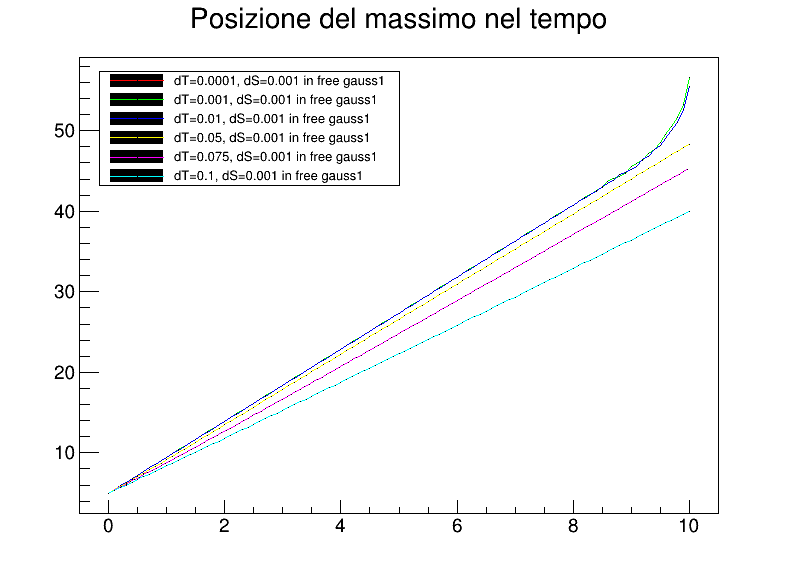
\includegraphics[width=\textwidth]{IMG/v_g1_0001}
		\caption[Differenze in 0.001]{Le differenze per $dS = 0.001$}
	\end{subfigure}
	~
	\begin{subfigure}[b]{0.3\textwidth}
		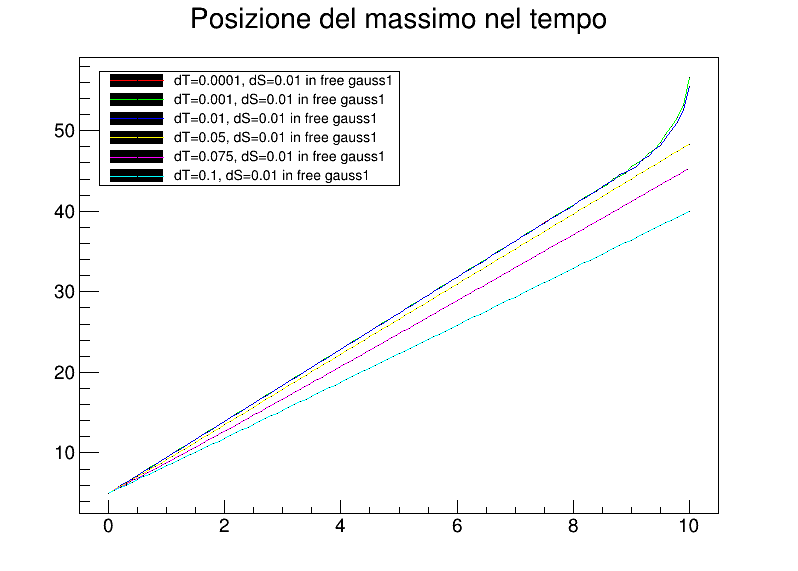
\includegraphics[width=\textwidth]{IMG/v_g1_001}
		\caption[Differenze in 0.01]{Le differenze per $dS = 0.01$}
	\end{subfigure}
	~
	\begin{subfigure}[b]{0.3\textwidth}
		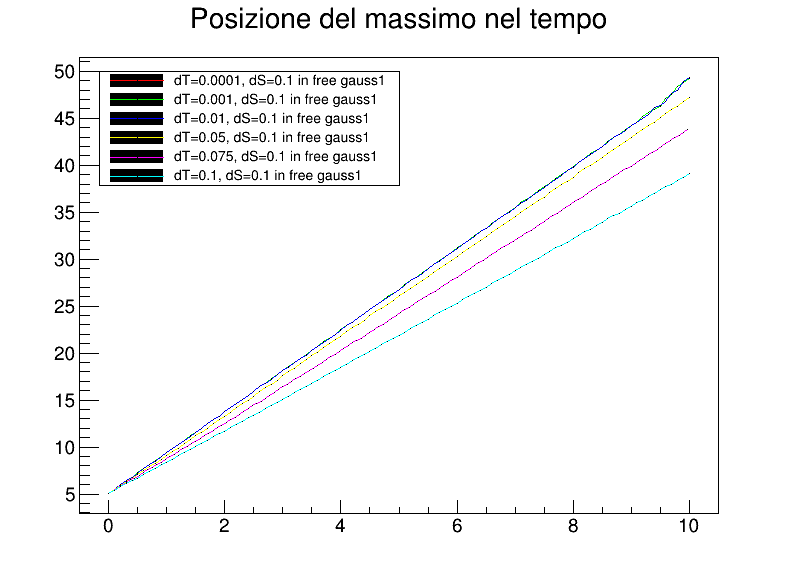
\includegraphics[width=\textwidth]{IMG/v_g1_01}
		\caption[Differenze in 0.1]{Le differenze per $dS = 0.1$}
	\end{subfigure}
	\caption{Le posizioni dei massimi nel tempo della simulazione a vari passi temporali  e spaziali}\label{fig:velocita}
\end{figure}

Prima di tutto effettuo diversi lanci per vedere come si comporta la simulazione al variare dei parametri.
Dai primi lanci capisco che devo scartare l'idea di usare un passo temporale grande in quanto ho notato che le funzioni d'onda vengono ``rallentate'', come si pu\`o vedere in \autoref{fig:velocita} le simulazioni con un passo temporale pi\`u grande di $0.01$ sono da scartare. Il punto in cui gli andamenti perdono l'andamento lineare e` dovuto al fatto che il pacchetto sta impattando contro il bordo del dominio e quindi inizia a rimbalzare e si iniziano a vedere le figure di interferenza.

%rifare tutto per verificare teoria!!!!!!!!!!!!!!!!!!!!!!!!!!!!!!!!!!!!!!!!!!!!!!!!!!!!!!!!!!!!!!!!!!!!!!!!!
%http://www.colorado.edu/physics/phys2170/phys2170_sp07/downloads/Gaussian.pdf
Analizzando meglio l'equazione svolgo i calcoli e mi aspetto che la simulazione ritorni:
\begin{equation}
%\Psi(x,t) = A(t)e^{-\frac{\lrt{x-x_0-\o t}^2}{2\sigma^2}}e^{ik\lrt{x-\o t}}
\Psi(x,t) = A(t)e^{-\frac{\lrt{x-x_0- v t}^2}{2\sigma(t)^2}}e^{ikx-\o t}
\end{equation}
dove $\o = \frac E\hbar$  e $v = \frac{p}{m} =\frac{\sqrt{2m E}}{m} $, ricordando che stiamo lavorando con pacchetti di onde piane monocromatici.
Quindi che i massimi delle onde da me simulate si spostino nel tempo seguendo la legge:
\begin{equation}
x_0(t) = x_0(0)+\sqrt{2\frac{E}{m}} t
\end{equation}
%%%%%%%%%%%%%%%%%%
%%non rispetta questo ma va confrontato con il fatto che invece rispetta la dispersione
\begin{figure}[hbt]
	\centering
	\begin{subfigure}[b]{0.3\textwidth}
		\begin{tikzpicture}[scale =0.66]
		\def \m {5};
		\begin{axis}[axis x line = center, axis y line = center, ylabel=v, ylabel style={left}, xlabel=E, xlabel style={below right}, xmin = 0, xmax = 208, ymin=-0.1,ymax =8.2, legend style={at={(1,0.1)},anchor=south east}]
		\addplot[domain=8:208, samples =501, orange]	plot[id=velm20]	function{sqrt(2*x/\m)};
		\addlegendentry{Teoria $m=5$}
		\addplot table[x=E,y=m5] {Dati/vel.tdt};
		\addlegendentry{$\Delta x =0.005$, $\Delta t = 0.01$}
		\addplot table[x=E,y=m5] {Dati/velprec.tdt};
		\addlegendentry{$\Delta x =0.001$, $\Delta t = 0.005$}
		\end{axis}
		\end{tikzpicture}
	\end{subfigure}
	~
	\begin{subfigure}[b]{0.3\textwidth}
		\begin{tikzpicture}[scale =0.66]
		\def \m {10};
		\begin{axis}[axis x line = center, axis y line = center, ylabel=v, ylabel style={left}, xlabel=E, xlabel style={below right}, xmin = 0, xmax = 208, ymin=-0.1,ymax =6.2, legend style={at={(1,0.1)},anchor=south east}]
		\addplot[domain=8:208, samples =501, orange]	plot[id=velm20]	function{sqrt(2*x/\m)};
		\addlegendentry{Teoria $m=10$}
		\addplot table[x=E,y=m10] {Dati/vel.tdt};
		\addlegendentry{$\Delta x =0.005$, $\Delta t = 0.01$}
		\addplot table[x=E,y=m10] {Dati/velprec.tdt};
		\addlegendentry{$\Delta x =0.001$, $\Delta t = 0.005$}
		\end{axis}
		\end{tikzpicture}
	\end{subfigure}
	~
	\begin{subfigure}[b]{0.3\textwidth}
		\begin{tikzpicture}[scale =0.66]
		\def \m {20};
		\begin{axis}[axis x line = center, axis y line = center, ylabel=v, ylabel style={left}, xlabel=E, xlabel style={below right}, xmin = 0, xmax = 208, ymin=-0.1,ymax =5.2, legend style={at={(1,0.1)},anchor=south east}]
		\addplot[domain=8:208, samples =501, orange]	plot[id=velm20]	function{sqrt(2*x/\m)};
		\addlegendentry{Teoria $m=20$}
		\addplot table[x=E,y=m20] {Dati/vel.tdt};
		\addlegendentry{$\Delta x =0.005$, $\Delta t = 0.01$}
		\addplot table[x=E,y=m20] {Dati/velprec.tdt};
		\addlegendentry{$\Delta x =0.001$, $\Delta t = 0.005$}
		\end{axis}
		\end{tikzpicture}
	\end{subfigure}
	\caption{Studio velocit\`a: si pu\`o osservare che con basse energie la simulazione tende a essere pi\`u fedele alla teoria.}\label{fig:simvel}
\end{figure}
Ho quindi verificato che la relazione funzionasse ma come si pu\`o osservare da \eqref{fig:simvel} la simulazione tende a essere pi\`u vicina alla teoria solo a basse energie o ad avvicinarsi di pi\`u aumentando la precisione.

\subsection{Lancio senza potenziale: errore}\label{sec:errore}
Ho deciso di definire un ``errore'' per capire quanto la simulazione possa essere andata a buon fine utilizzando la norma della funzione, ricordando che le funzioni d'onda sono $L^2$ e quindi la loro norma \`e  $\lr||f^2=\int_X\lr||f^2d\mu$.
Per calcolarlo ho utilizzato la definizione dell'integrale discreto di Simpson, il che mi limita a poter fare solo simulazioni con un numero di passi pari (e in particolare multipli di 4 per aver un integrale preciso anche quando calcolo l'integrale solo nella prima o seconda met\`a del dominio) nello spazio.

Nella simulazione blocco il calcolo se la norma della funzione si discosta troppo dalla norma delle condizioni iniziali, il limite viene scelto nel file delle impostazioni.

A questo punto ho  guardato l'errore nelle simulazioni, scartando a priori i passi temporali pi\`u grandi di $0.01$, \autoref{fig:fullErr} e \ref{fig:fullErrzoom}.

\begin{figure}[hbt]
  \centering
  \begin{subfigure}[b]{0.45\textwidth}
    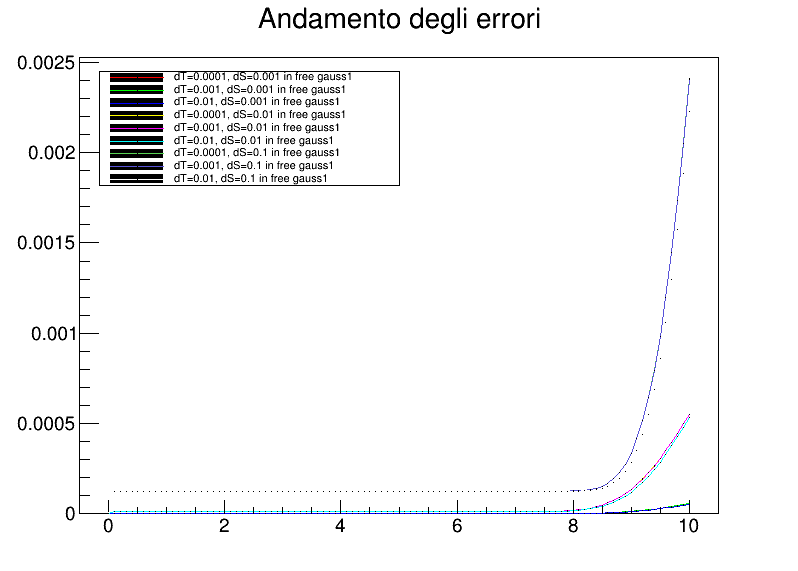
\includegraphics[width=\linewidth]{IMG/e_g1full}
    \caption[Errori completo]{Il grafico completo degli errori}\label{fig:fullErr}
  \end{subfigure}
  ~
  \begin{subfigure}[b]{0.45\textwidth}
    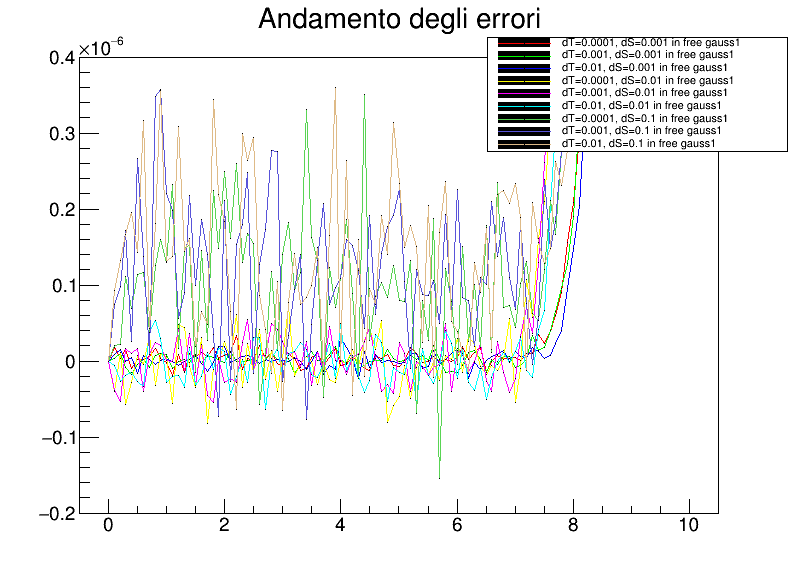
\includegraphics[width=\linewidth]{IMG/e_g1res}
    \caption[Errori zoom]{Zoom per mostrare dove la riflessione non ha influenza}\label{fig:fullErrzoom}
  \end{subfigure}
  \caption[Errori completo]{Il grafico degli errori, si vede anche quanto la riflessione influisca sul modulo della funzione.}\label{fig:Err}
\end{figure}

Quindi ho fatto una simulazione diminuendo il tempo massimo a $6$ in modo da non avere a che fare con l'esplosione dell'errore dovuta al limite del dominio. e cosi` da poter osservare quale fosse il miglior passo spaziale. Ho fatto i lanci con due diverse condizioni iniziali (gaussiana con $\sigma$ $1$ e $2$). 

\begin{figure}[htb]
  \centering
  \begin{subfigure}[b]{0.45\textwidth}
    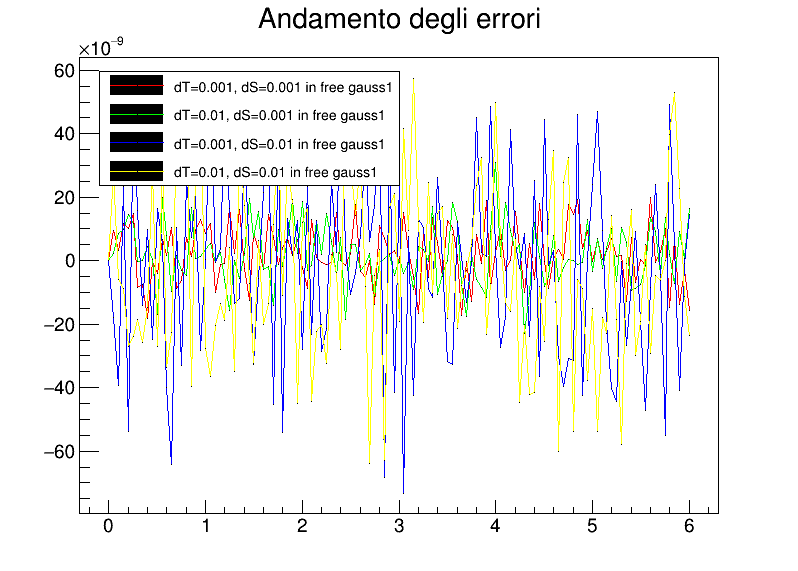
\includegraphics[width=\textwidth]{IMG/eChoosy1}
    \caption{CI: gaussiana($\sigma=2$)}
  \end{subfigure}
  ~
  \begin{subfigure}[b]{0.45\textwidth}
    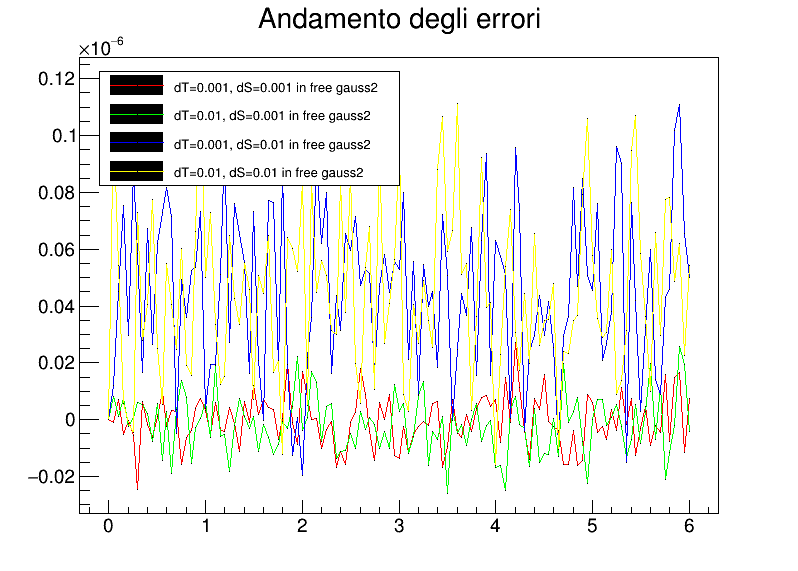
\includegraphics[width=\textwidth]{IMG/eChoosy2}
    \caption{CI: gaussiana($\sigma=2$)}
  \end{subfigure}
  \caption{I passi che mi sembravano pi\`u opportuni a confronto}\label{fig:SceltaErrori}
\end{figure}

Osservando \autoref{fig:SceltaErrori} utilizzare come passi spaziali e temporali valori compresi tra $0.01$ e $0.001$ ha un buon rapporto ``errore sulla simulazione/peso sul calcolatore'', in particolare si nota che il passo spaziale influenza di pi\`u l'errore. Ho scelto di continuare con $dT = 0.01$ e $dS = 0.005$ in quanto hanno errore molto simile a $dS = 0.001$ (\autoref{fig:sceltaPassi}) ma sono pi\`u rapidi nei calcoli (sulla mia macchina).

\begin{figure}[hbt]
  \centering
  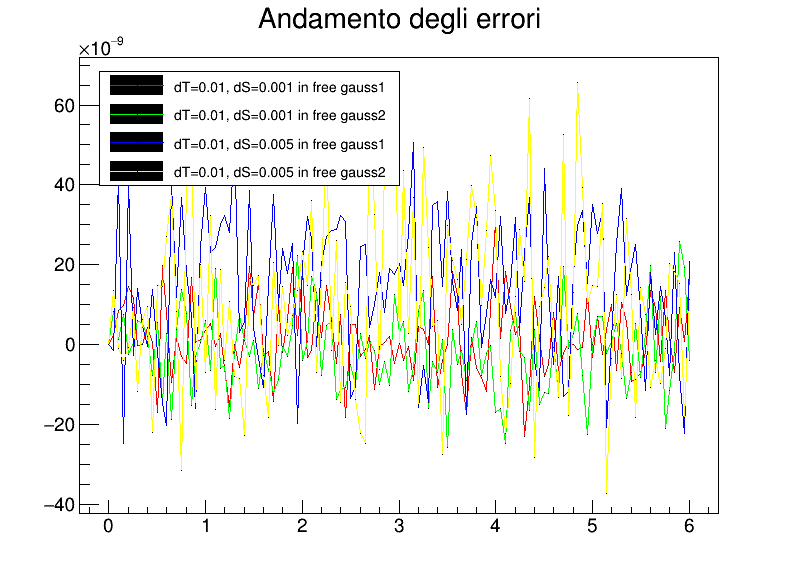
\includegraphics[width=0.7\textwidth]{IMG/sceltaPassi}
  \caption[Scelta Passi]{Gli errori dei passi che ritengo pi\`u convenienti}\label{fig:sceltaPassi}
\end{figure}

\subsection{Dispersione dei pacchetti d'onda}
%pacchetti di Airy non disperdono-> provare
\begin{figure}[htb]
  \centering
  \foreach \x in {1,3,7,10}{
    \begin{subfigure}[b]{0.4\textwidth}
      \centering
      \includegraphics[width=\textwidth]{IMG/dispersione_\x}
    \end{subfigure}
    \ifthenelse{\equal{\x}{3}}{\\}{~} 
  }
  \caption{La dispersione delle gaussiana a $\sigma =1$, in verde le condizioni iniziali}\label{fig:dispersione}
\end{figure}

La prima cosa che si pu\`o osservare nelle simulazioni (e in particolare in \autoref{fig:dispersione}) \`e la dispersione dell'onda, ovvero il pacchetto si allarga nel tempo. Questa \`e una caratteristica dell'equazione di Schr\"{o}dinger, in quanto la sua forma \`e appunto quella di una qualsiasi equazione che descriva la dispersione.

Voglio calcolare la teoria di questo fenomeno per poterlo confrontare con i risultati che ho ottenuto nelle prime simulazioni.
Per ottenere la soluzione dell'equazione con condizioni iniziali $\psi\lrt{x,0}=e^{-\frac{x^2}{2\sigma^2}}$ si passa dalla trasformata di Fourier spaziale $\hat\psi\lrt{x,0}=\sqrt{2\pi\sigma^2} e^{-\frac{k^2 \sigma^2}2}$, che porta ad avere la funzione, con dipendenza temporale:

\begin{equation}
  \hat{\psi}\lrt{k,t} = \sqrt{2\pi\sigma^2} e^{-\frac{k^2 \sigma^2}2} e^{-i\frac E\hbar t} =
  \sqrt{2\pi\sigma^2} e^{-\frac{k^2 \sigma^2}2} e^{-i\frac {\hbar^2 k^2/2m}\hbar t} = 
  \sqrt{2\pi\sigma^2} e^{-k^2\frac{\lrt{\sigma^2+i\hbar t/m}}2 }
\end{equation}
e poi ritrasformando:
\begin{equation}
  \psi\lrt{x,t} = \frac{\sigma}{\sqrt{\sigma^2 + i\hbar t /m}}
  e^{-\frac{k^2}{2\lrt{\sigma + i\hbar t/m}}}
\end{equation}
ora calcolo il valore assoluto della funzione:
\begin{equation}
  \lr||{\psi\lrt{x,t}} = \frac{\sigma}{\sqrt[4]{\sigma^4 + \lrt{\hbar t /m}^2}}
  e^{-\frac{k^2}2\frac{\sigma^2}{\sigma^4 + \lrt{\hbar t /m}^2}} = \sqrt{\frac{\sigma_0}{\sigma(t)}}e^{-\frac{k^2}{2\sigma^2(t)}}
\end{equation}

E, chiamando $\sigma_0$ il valore assegnato nelle condizioni iniziali, mi aspetto dalla simulazione che $\sigma$ evolva come
\begin{equation}\label{eq:sigmat}
  \sigma(t) = \sqrt{\frac{\sigma_0^4+\lrt{\frac\hbar m t}^2}{\sigma_0^2}}
\end{equation}

Ho fatto diversi fit, sul parametro $\sigma$, con diverse masse e diversi valori di $\sigma$ iniziali, utilizzando come funzione da fittare \eqref{eq:sigmat}. L'algoritmo sembra rispettare la dispersione,  come si pu\`o vedere in \autoref{fig:dispersioneFitSigma1}, in
\autoref{fig:dispersioneFitSigma4} e in \autoref{fig:dispersioneFitE} dove la funzione ha energia diversa da 0

\begin{figure}[htb]
  \centering
  \begin{subfigure}[b]{0.3\textwidth}
    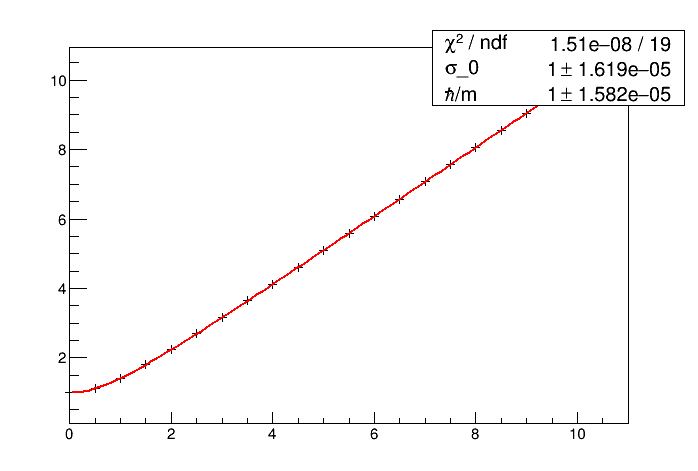
\includegraphics[width=\linewidth]{IMG/dispersione_p}
    \caption{$\sigma_0=1$, $m=1$}
  \end{subfigure}
  ~
  \begin{subfigure}[b]{0.3\textwidth}
    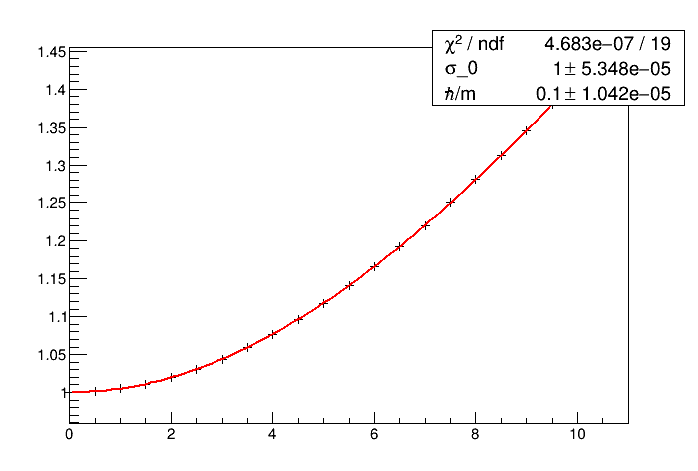
\includegraphics[width=\linewidth]{IMG/dispersione_m10}
    \caption{$\sigma_0=1$, $m=10$}
  \end{subfigure}
  ~
  \begin{subfigure}[b]{0.3\textwidth}
    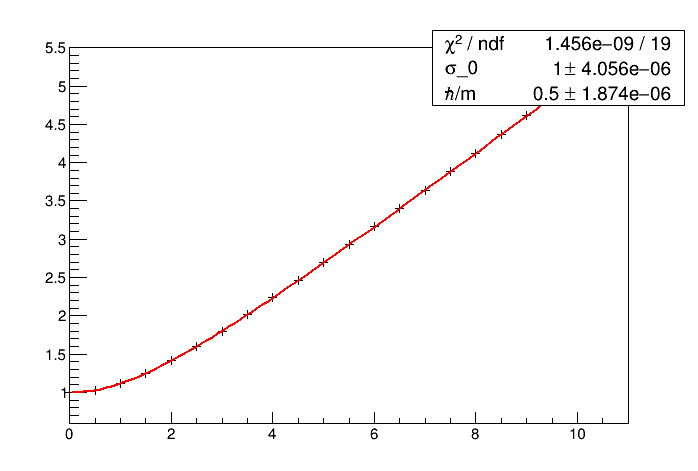
\includegraphics[width=\linewidth]{IMG/dispersione_m2}
    \caption{$\sigma_0=1$, $m=2$}
  \end{subfigure}
  \caption{Alcuni fit dell'andamento della dispersione}\label{fig:dispersioneFitSigma1}
\end{figure}

\begin{figure}[htb]
  \centering
  \begin{subfigure}[b]{0.3\textwidth}
    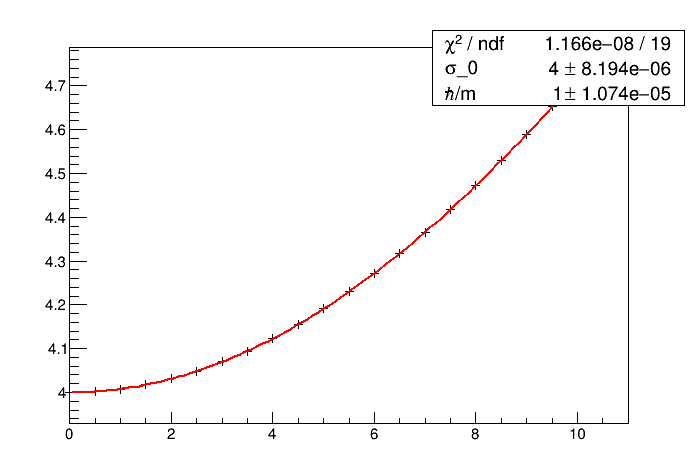
\includegraphics[width=\linewidth]{IMG/dispersione_m1s4}
    \caption{$\sigma_0=4$, $m=1$}
  \end{subfigure}
  ~
  \begin{subfigure}[b]{0.3\textwidth}
    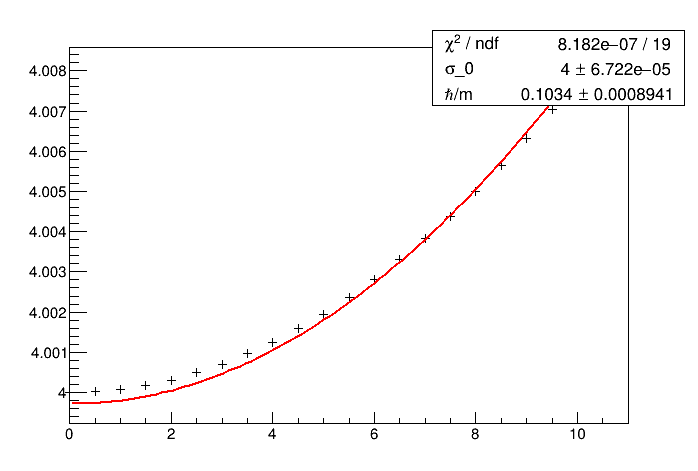
\includegraphics[width=\linewidth]{IMG/dispersione_m10s4}
    \caption{$\sigma_0=4$, $m=10$}
  \end{subfigure}
  ~
  \begin{subfigure}[b]{0.3\textwidth}
    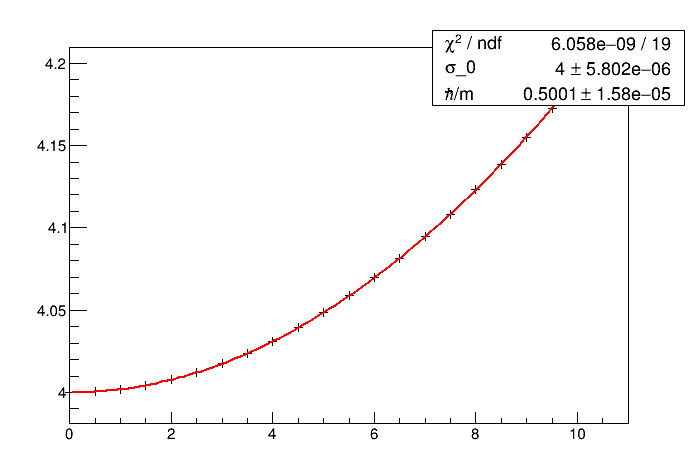
\includegraphics[width=\linewidth]{IMG/dispersione_m2s4}
    \caption{$\sigma_0=4$, $m=2$}
  \end{subfigure}
  \caption{Alcuni fit dell'andamento della dispersione}\label{fig:dispersioneFitSigma4}
\end{figure}

\begin{figure}[htb]
  \centering
  \begin{subfigure}[b]{0.3\textwidth}
    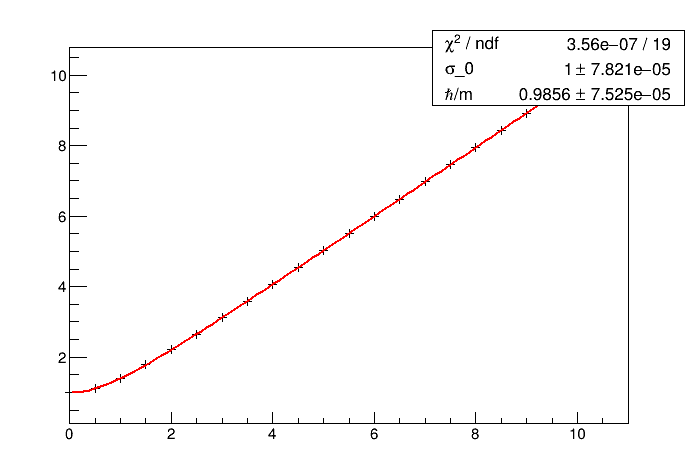
\includegraphics[width=\linewidth]{IMG/dispersione_m1s1e10}
    \caption{$\sigma_0=1$, $m=1$, con $E=10$}
  \end{subfigure}
  ~
  \begin{subfigure}[b]{0.3\textwidth}
    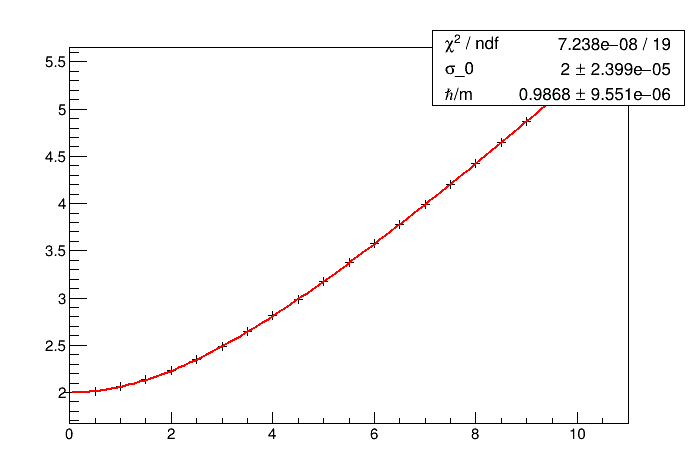
\includegraphics[width=\linewidth]{IMG/dispersione_m1s2e10}
    \caption{$\sigma_0=2$, $m=1$, con $E=10$}
  \end{subfigure}
  ~
  \begin{subfigure}[b]{0.3\textwidth}
    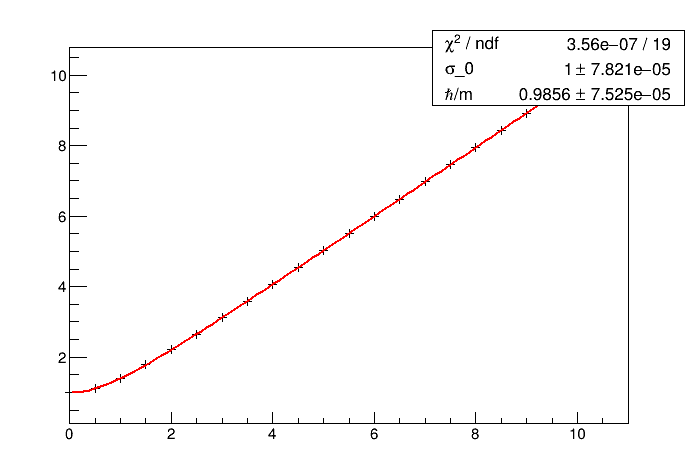
\includegraphics[width=\linewidth]{IMG/dispersione_m1s1e10}
    \caption{$\sigma_0=4$, $m=1$, con $E=10$}
  \end{subfigure}
  \caption{Alcuni fit dell'andamento della dispersione}\label{fig:dispersioneFitE}
\end{figure}

\subsection{La forma delle condizioni iniziali}
Ho effettuato i test precedenti utilizzando come condizione iniziale un pacchetto d'onda gaussiano. Per effetto della dispersione \`e un pacchetto deltiforme che nel tempo si \`e disperso allargandosi in una gaussiana.

Ho provato  ad utilizzare una forma differente per il pacchetto: la funzione ``bump'':
\begin{figure}[hbt]
	\centering
	\begin{tikzpicture}[scale=0.5]
	\begin{axis}[axis x line = center, axis y line = center, xmin = -0.1, xmax = 4.1, ymin=-0.1,ymax =1.5]
	\addplot[domain=-0.1:4.1, samples =501, red]	plot[id=bumpl1]	function{(abs(x-1)<1)? exp(1)*exp(-1/(1-(x-1)*(x-1))):0};
	\addlegendentry{$a=1$, $b=1$}
	\addplot[domain=-0.1:4.1, samples =501, blue]	plot[id=bumpl1]	function{(abs(x-1)<2)? exp(1)*exp(-4/(4-(x-1)*(x-1))):0};
	\addlegendentry{$a=1$, $b=2$}
	\addplot[domain=-0.1:4.1, samples =501, green]	plot[id=bumpl1]	function{(abs(x-3)<1)? exp(-1/(1-(x-3)*(x-3))):0};
	\addlegendentry{$a=3$, $b=1$ non moltiplicata per $e$}
	\end{axis}
	\end{tikzpicture}
	\caption{Alcuni esempi della funzione bump}\label{fig:bump}
\end{figure}

\begin{equation}
bump = \lrt{x} = \lr\{.{\begin{array}{lr}
	e^{-\frac{b^2}{b^2-\lrt{x-a}^2}}&\text{per }\lr||{x-a}<b\\
	0&\text{altrove}
	\end{array}}
\end{equation}

Il ''bump`` \`e una funzione di test quindi \`e definita differente da 0 solo in un intervallo aperto, ed ha la caratteristica di avere tutte le derivate continue, questo mi permetterebbe di ignorare completamente le condizioni al contorno quando la funzione si trova lontano dai bordi della simulazione.
Inoltre moltiplico il risultato per $e$ per avere un pacchetto con il massimo alto $1$, vedi \autoref{fig:bump}.

\begin{figure}[hbt]
	\centering
	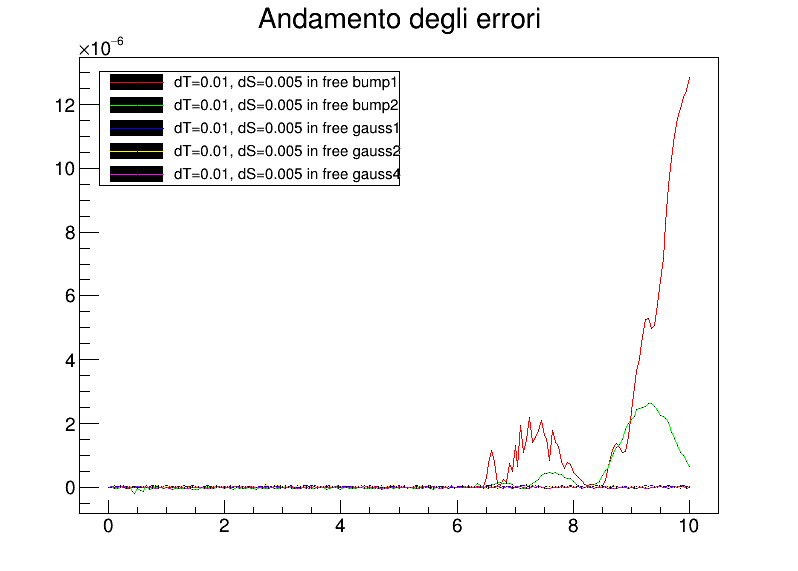
\includegraphics[width=0.5\linewidth]{IMG/testbump}
	\caption[Errore Bump]{l'evoluzione dell'errore del ``bump'' confrontata con quella di un pacchetto gaussiano}\label{fig:testBump}
\end{figure}

A questo punto simulo il pacchetto e confronto l'errore con uno gaussiano. Come si pu\`o vedere dalla \autoref{fig:testBump} non \`e una buona idea.

L'errore cresce molto verso la fine della simulazione, questo potrebbe essere dovuto al fatto che sta impattando contro i limiti del dominio, inoltre se si osserva l'evoluzione della funzione si vede che perde praticamente subito la forma iniziale e quindi anche i vantaggi di avere le code pari a 0.
\begin{figure}[htb]
	\centering
	\begin{subfigure}[b]{0.49\textwidth}
		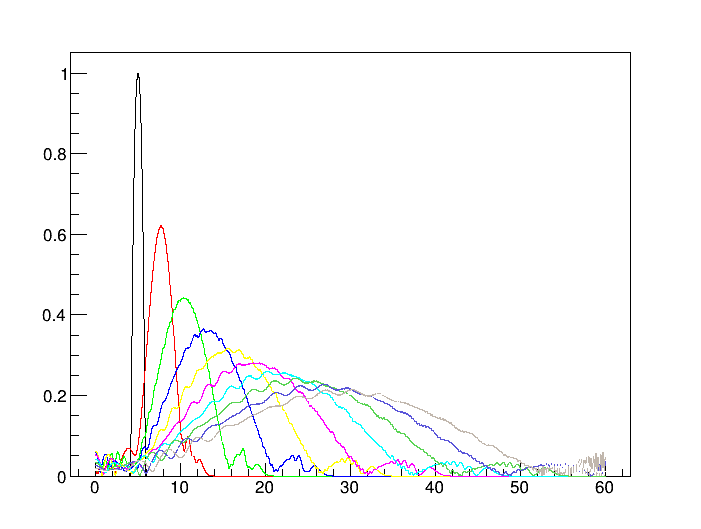
\includegraphics[width=\textwidth]{IMG/bumpDisp1.png}
		\caption{larghezza 1}
	\end{subfigure}
	~
	\begin{subfigure}[b]{0.49\textwidth}
		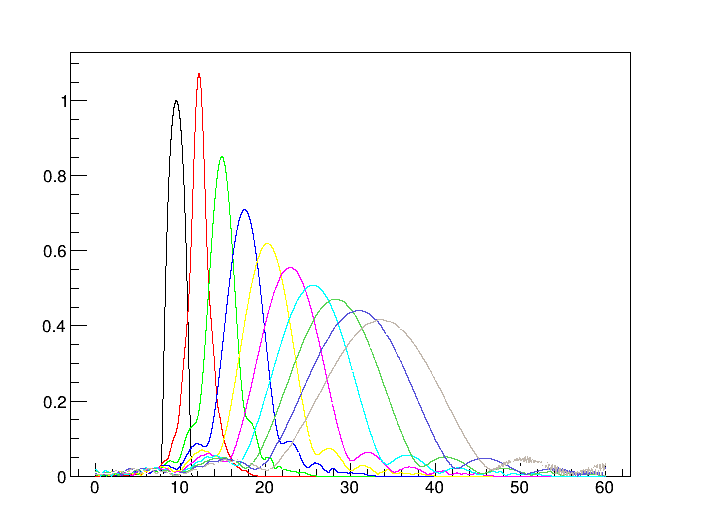
\includegraphics[width=\textwidth]{IMG/bumpDisp2.png}
		\caption{larghezza 2}
	\end{subfigure}
	\caption{L'evoluzione del ``bump'', le ``increspature'' sull'onda che si vedono ai lati sono le figure di interferenza dovute alla riflessione}
\end{figure}

A questo punto l'idea migliore per il pacchetto d'onda sembra essere la gaussiana.


\subsection{Condizioni al contorno}
Quello che vorrei simulare \`e un pacchetto d'onda che sia partito da $-\infty$ e arrivi nel ``punto interessante'', l'area che osservo nella simulazione, e poi prosegua fino all'infinito (o venga eventualmente riflesso).

Per quanto riguarda le condizioni al contorno ho avuto le seguenti idee:
\begin{itemize}
\item Non tengo conto delle condizioni al contorno, faccio in modo di usare pacchetti d'onda ristretti e blocco la simulazione quando questa va ad  avvicinarsi troppo ai bordi.
\item Uso una forma d'onda tale per cui conosco la funzione e la sua derivata in ogni punto
\item Emulo un ambiente chiuso (con ai lati muri di potenziale alti $\infty$)
\end{itemize}
La prima ipotesi \`e stata quella che ho usato in tutte le prove che ho effettuato prima di iniziare a raccogliere dati, considerando 0 il valore della funzione negli estremi.

Per la seconda ipotesi dovrei usare come condizione iniziale una funzione e calcolarne la derivata per ogni passo negli estremi. Ma pacchetti d'onda si disperdono e tendono ad allargarsi, per cui se,  per esempio avessi un pacchetto d'onda generico ($\Psi(x,t) = e^{ikx} \psi(x,t)$), la relazione dovrebbe essere $\partial_x \Psi(x,t) = ik \Psi(x,t) + e^{ikx}\partial_x\psi(x,t)$ e potrei quindi utilizzare le CC di Robin. Ma doveri conoscere come la funzione si disperde nel tempo e ricalcolare quindi  ad ogni passo le condizioni al contorno ed applicarle. Questo per\`o mi porterebbe a svariati problemi quali l'incertezza che la simulazione e la teoria siano esattamente parallele sulla dispersione, il che porterebbe ad altri errori, ed il fatto che molto probabilmente sarebbe poco efficiente dal punto di vista della performance del calcolo.

La terza idea equivale a utilizzare Dirichlet con il valore della funzione pari a 0 nei bordi questo simula un pozzo con pareti di potenziale infinito.

%Per cui ho deciso di ricercare un'idea che simulasse l'assenza di vincoli: ho trovato le cosiddette condizioni al contorno trasparenti.
%Ma ho lasciato perdere data la loro complessit\`a e il poco tempo a mia disposizione, in quanto utilizza la trasformazione Z

\subsection{Prime Conclusioni}
Dopo i primi esperimenti sono arrivato a queste conclusioni:
\begin{itemize}
\item Far\`o le simulazioni utilizzando una gaussiana come forma del pacchetto d'onda, perch\'e mantiene la propria forma.
\item Per contenere la dispersione dell'onda, vista la forma di \eqref{eq:sigmat} posso scegliere di utilizzare un $\sigma_0$ grande oppure una massa grande
  \begin{itemize}
  \item con una massa grande per avere la stessa velocit\`a di gruppo devo aumentare l'energia, ma in compenso posso utilizzare dei $\sigma_0$ piuttosto piccoli e quindi questo mi rende pi\`u semplice il compito di fare confronti tra due parti di spazio limitate per analizzare la trasmissivit\`a delle barriere di potenziale
  \item con $\sigma_0$ grande il pacchetto d'onda  non ha bisogno di una grande energia per muoversi, ma il fatto che esso sia esteso pu\`o comportare problemi per esempio quando si riflette contro un potenziale o quando lo attraversa o nel momento di definire le condizioni iniziali, perch\'e rischio di sovrapporre l'onda al potenziale.
  \end{itemize}
\item Come condizioni al contorno simuler\`o la scatola chiusa con pareti infinite, sebbene una prima idea fosse quella di utilizzare le condizioni ``trasparenti'', ma questo oltre ad appesantire il programma farebbe uscire il pacchetto d'onda dalla mia ``zona d'osservazione'' e quindi non sarei pi\`u in grado di fare l'integrale di tutto il pacchetto (comprese le sue riflessioni e i pezzi in cui si \`e diviso).
\item Per ritardare il pi\`u possibile l'interazione con le condizioni al contorno devo aumentare l'intervallo spaziale se aumento il tempo della simulazione
\item Guardando i risultati che ho osservato con guardando la velocit\`a devo limitare l'energia dei pacchetti d'onda al di sotto di $E=25$
\end{itemize}

Con queste conclusioni in mano mi appresto a simulare le situazioni per cui ho progettato questo algoritmo e confrontarle con la teoria.

\section{Dati e analisi}
Con le impostazioni che ho ricavato nella sezione precedente ho quindi proceduto con la simulazione del comportamento delle onde in presenza di vari potenziali.
\subsection{Il salto di potenziale}
Il primo potenziale che analizzo \`e il salto di potenziale, posiziono un gradino a met\`a del dominio e variandone l'altezza ne calcolo il coefficiente di trasmissivit\`a.

\begin{equation}\label{eq:Salto}
  \lr\{.{\begin{array}{lr}
      V_0& x>a\\
      0&\text{altrove}
  \end{array}}
\end{equation}


Quindi proseguiamo ed eseguiamo delle simulazioni. Per confrontare i risultati delle simulazioni con la teoria ho sostituito in \eqref{eq:riflessioneStepvanilla} $V =  E/x$ notando che il risultato non dipende dall'energia:

\begin{equation}
\lr\{.{\begin{array}{l}
	R =  \frac{2 x -1 -2 \sqrt{x\lrt{x-1}}}{2x -1 +2 \sqrt{x\lrt{x-1}}}\\
	T =  \frac{4 \sqrt{x\lrt{x-1}}}{2x -1 +2 \sqrt{x\lrt{x-1}}}
	\end{array}}
\end{equation}

Nelle simulazioni i lanci sono stati fatti con pacchetti gaussiani inizialmente con $\sigma=0.5$, energia $100$ e massa $10$. Il potenziale \`e stato impostato perch\'e il salto fosse al centro del dominio e con altezza diversa per ogni lancio e ho analizzato l'andamento temporale del rapporto tra l'integrale su tutto il dominio e quello fatto nella prima met\`a.
Ho deciso di usare come coefficiente di riflessione il valore del peso dell'integrale quando questo si \`e stabilizzato.
Dall'andamento nel tempo si pu\`o vedere un piccolo abbassamento quando l'onda impatta il potenziale per le barriere pi\`u alte, prima di venire riflessa all'indietro penetra leggermente nell'area classicamente vietata.

\begin{figure}[htb]
  \centering
  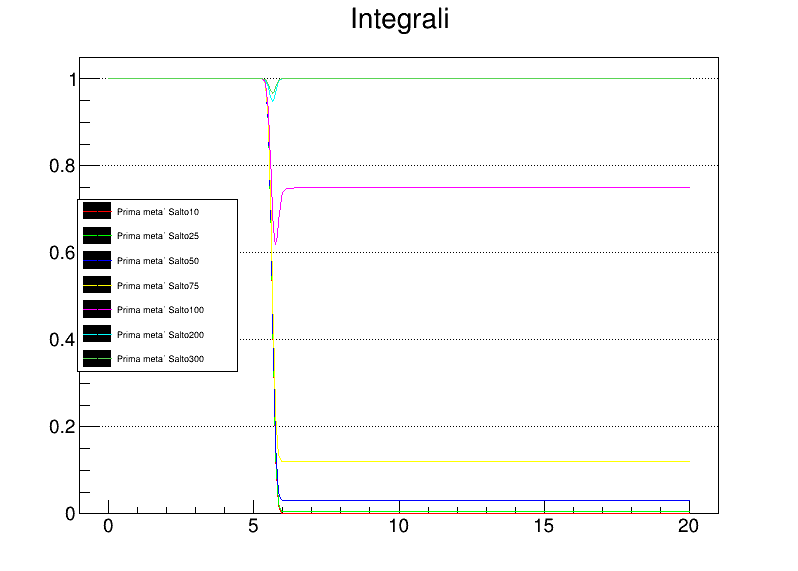
\includegraphics[width=0.7\linewidth]{IMG/SaltoR}
  \caption{I pesi dell'integrale della prima met\`a del dominio per $\sigma=0.5$. Dove c'\`e riflessione si nota una penetrazione parziale dell'onda nella seconda met\`a del dominio seguita dalla riflessione}\label{fig:SaltoR}%RIFARE CON ENERIGA APPROPRIATA
\end{figure}

Come si pu\`o notare dalla \autoref{tab:SaltoDati} sebbene stia simulando un pacchetto d'onda in movimento e non un un'onda piana il peso dei coefficienti ricalca abbastanza bene i coefficienti teorici, e sembra avvicinarli di pi\`u man mano che allargo il pacchetto. Notare che la simulazione si allontana dalla teoria per le onde piane pi\`u si \`e vicini al regime in cui il potenziale \`e maggiore dell'energia dell'onda.

\begin{figure}[hbt]
	\centering
	\begin{subfigure}[b]{0.49\textwidth}
  \begin{tikzpicture}
  \def \En {10};
  \begin{axis}[axis x line = center, axis y line = center, ylabel=R, ylabel style={left}, xlabel=E/V, xlabel style={below right}, xmin = -0.1, xmax = 10.1, ymin=-0.1,ymax =1.1]
  \addplot table[x=ev,y=E\En] {Dati/saltos05.tdt};%{Dati/Salto.tdt};
  \addlegendentry{$\sigma=0.5$}
  	\foreach \sig in {1,2,4}{
  		\addplot table[x=ev,y=E\En] {Dati/saltos\sig.tdt};
  		\edef\temp{\noexpand\addlegendentry{$\sigma = \sig$}}
  		\temp
  	}
  \addplot[domain=0:10, samples =501, green]	plot[id=Refl2]	function{\Rjump(x)};
  \addlegendentry{teoria}
  \end{axis}
  \end{tikzpicture}
	\end{subfigure}
	~
	\begin{subfigure}[b]{0.49\textwidth}
  \begin{tikzpicture}
  \def \sig {2};
  \begin{axis}[axis x line = center, axis y line = center, ylabel=R, ylabel style={left}, xlabel=E/V, xlabel style={below right}, xmin = -0.1, xmax = 10.1, ymin=-0.1,ymax =1.1]
  	\foreach \E in {10,15,20,25}{
		\addplot table[x=ev,y=E\E] {Dati/saltos\sig.tdt};
		\edef\temp{\noexpand\addlegendentry{$E=\E$}}
		\temp
	}
  \addplot[domain=0:10, samples =501, green]	plot[id=Refl2]	function{\Rjump(x)};
  \addlegendentry{teoria}
  \end{axis}
  \end{tikzpicture}
	\end{subfigure}
  \caption{La visualizzazione dei dati e il confronto con la teoria, il primo grafico fatto con $E=10$, il secondo con $\sigma = 2$}
\end{figure}

Dai grafici si nota che se $\sigma$ \`e piccolo c'\`e una tendenza  a deviare dal comportamento teorico, mentre variando l'energia non sembrano esserci differenze

%%%%%%%%%%%%%%%%%%%%%%%%%%%%%%%%%%%%%%%%%%%%%%%%%%%%%%%%%%%%%%%%%%%%%%%%%%%%%%%%%%%%%%%%%%%%%%%%%
%%%%%%%%%%%%%%%%%%%%%%%%%%%%%%%%%%%%%%%%%%%%%%%%%%%%%%%%%%%%%%%%%%%%%%%%%%%%%%%%%%%%%%%%%%%%%%%%%
%%%%%%%%%%%%%%%%%%%%%%%%%%%%%%%%%%%%%%%%%%%%%%%%%%%%%%%%%%%%%%%%%%%%%%%%%%%%%%%%%%%%%%%%%%%%%%%%%
%%%%%%%%%%%%%%%%%%%%%%%%%%%%%%%%%%%%%%%%%%%%%%%%%%%%%%%%%%%%%%%%%%%%%%%%%%%%%%%%%%%%%%%%%%%%%%%%%
\subsection{La barriera rettangolare}
Ho quindi simulato il comportamento dell'onda in presenza di una barriera rettangolare:

\begin{equation}\label{eq:Barriera}
  \lr\{.{\begin{array}{lr}
      V_0& 0<x<a\\
      0&\text{altrove}
  \end{array}}
\end{equation}

Ho svolto la teoria nella \autoref{sec:BarrieraCalc}.
I grafici che in seguito riporter\`o mostrano il valore del modulo della forma d'onda contenuta nella parte di dominio a sinistra della barriera che corrisponde al coefficiente di riflessione della teoria per le onde piane. I grafici sono disegnati in funzione del rapporto $ E/V$, dato che nelle simulazioni ho variato il valore del potenziale ho sostituito $V = E/x$ in \eqref{eq:riflessionevanilla} per poterla visualizzare come confronto teorico:

\begin{equation}
R\lrt{m,E,x} = \lr\{.{\begin{array}{lr}
	\lrt{1+4 \frac{\lrt{x-x^2}}{\sinh^2\lrt{a \sqrt{2m E\lrt{1/x-1}}}}}^{-1} & 0<x<1 \\
	\lrt{1+\frac{2}{ a^2 m E}}^{-1}                                             & x=1 \\
	\lrt{1+4 \frac{\lrt{x^2 - x}}{\sin^2\lrt{a \sqrt{2m E\lrt{1-1/x}}}}}^{-1} & x>1
	\end{array}}
\end{equation}

%\begin{figure}[hbt]
%	\centering
%	\begin{tikzpicture}
%	\begin{axis}[axis x line = center, axis y line = center, ylabel=R, ylabel style={left}, xlabel=E/V, xlabel style={below right}, xmin = -0.1, xmax = 3.1, ymin=-0.1,ymax =1.1]
%	\foreach \a/\En/\mycol in {2/10/red,2/15/blue,4/10/green,4/15/orange}{
%		\addplot[domain=0.1:4, samples =501, \mycol]	gnuplot	{\Rbarrier(x,10,\En,\a)};
%		\edef\temp{\noexpand\addlegendentry{$a=\a$, $E=\En$}}
%		\temp
%	}
%%	\def \a {2}
%%	\def \En{10}
%%	\addplot[domain=0.1:4, samples =501, red]	gnuplot	{\Rbarrier(x,10,\En,\a)};
%%	\addlegendentry{$a=\a$, $E=\En$}
%%	\def \En{15}
%%	\addplot[domain=0.1:4, samples =501, blue]	gnuplot	{\Rbarrier(x,10,\En,\a)};
%%	\addlegendentry{$a=\a$, $E=\En$}
%%	\def \a {4}
%%	\def \En{10}
%%	\addplot[domain=0.1:4, samples =501, green]	gnuplot	{\Rbarrier(x,10,\En,\a)};
%%	\addlegendentry{$a=\a$, $E=\En$}
%%	\def \En{15}
%%	\addplot[domain=0.1:4, samples =501, orange]	gnuplot	{\Rbarrier(x,10,\En,\a)};
%%	\addlegendentry{$a=\a$, $E=\En$}
%	\end{axis}
%	\end{tikzpicture}
%	\caption{La teoria per alcuni valori di $E$ e di $a$, tenendo fissa la massa a $m=5$}
%\end{figure}

\begin{figure}[hbt]
  \centering
  \begin{tikzpicture}
    \def \a {2}
    \begin{axis}[axis x line = center, axis y line = center, ylabel=R, ylabel style={left}, xlabel=E/V, xlabel style={below right}, xmin = -0.1, xmax = 10.1, ymin=-0.1,ymax =1.1]
      \foreach \sig in {0.5,1,2,4}{
      	\addplot table[x=ev,y=s\sig] {Dati/Barriera_a1.tdt};
      	\edef\temp{\noexpand\addlegendentry{$\sigma = \sig$}}
      	\temp
      }
      \addplot[domain=0.1:10, samples =501, red]	gnuplot	{\Rbarrier(x,10,5,1)};
      \addlegendentry{teoria $a=2$ }
    \end{axis}
  \end{tikzpicture}
  \caption{La visualizzazione dei dati e il confronto con la teoria, con $E=5$, $m=10$ e $a=1$}\label{fig:Barriera}
\end{figure}

\begin{figure}[hbt]
  \centering
  \begin{subfigure}[b]{0.49\textwidth}
    \begin{tikzpicture}
      \begin{axis}[axis x line = center, axis y line = center, ylabel=R, ylabel style={left}, xlabel=E/V, xlabel style={below right}, xmin = 1.9, xmax = 4.1, ymin=-0.001,ymax = 0.11]
\foreach \sig in {0.5,1,2,3}{
	\addplot table[x=ev,y=s\sig] {Dati/DataOsc2.tdt};
	\edef\temp{\noexpand\addlegendentry{$a=2$, $\sigma=\sig$}}
	\temp
}
      \def \a {2};
      \def \m {10};
      \def \En {15};
	\addplot[domain=2:4, samples =501, blue]	plot[id=MRefl2z]	function{\Rbarrier (x,\m,\En,\a)};
	\addlegendentry{teoria a=\a}
	\addplot[domain=2:4, samples =501, red]	plot[id=Refl2]	function{\Rjump (x)};
	\addlegendentry{teoria scalino}
      \end{axis}
    \end{tikzpicture}
  \end{subfigure}
  ~
  \begin{subfigure}[b]{0.49\textwidth}
    \begin{tikzpicture}
      \def \a {2}
      \begin{axis}[axis x line = center, axis y line = center, ylabel=R, ylabel style={left}, xlabel=E/V, xlabel style={below right}, xmin = 1.9, xmax = 4.1, ymin=-0.001,ymax = 0.11]
	\foreach \sig in {4,5,6,7}{
		\addplot table[x=ev,y=s\sig] {Dati/DataOsc2.tdt};
		\edef\temp{\noexpand\addlegendentry{$a=2$, $\sigma=\sig$}}
	  \temp
	}
      \def \a {2};
      \def \m {10};
      \def \En {15};
      \addplot[domain=2:4, samples =501, blue]	plot[id=MRefl2z]	function{\Rbarrier (x,\m,\En,\a)};
      \addlegendentry{teoria a=\a}
	\addlegendentry{teoria a=\a}
      \end{axis}
    \end{tikzpicture}
  \end{subfigure}
  \caption{I dati tra 2 e 4 per una barriera larga 2, con $E=15$}\label{fig:Osc2}
\end{figure}


\begin{figure}[hbt]
  \centering
  \begin{subfigure}[b]{0.49\textwidth}
    \begin{tikzpicture}
      \def \a {4}
      \begin{axis}[axis x line = center, axis y line = center, ylabel=R, ylabel style={left}, xlabel=E/V, xlabel style={below right}, xmin = 1.9, xmax = 4.1, ymin=-0.001,ymax = 0.11]
            \foreach \sig in {0.5,1,2,3}{
            	\addplot table[x=ev,y=s\sig] {Dati/data.tdt};
            	\edef\temp{\noexpand\addlegendentry{$a=2$, $\sigma=\sig$}}
            	\temp
            }
      \def \a {4};
      \def \m {10};
      \def \En {15};
      \addplot[domain=2:4, samples =501, blue]	plot[id=MRefl2z]	function{\Rbarrier (x,\m,\En,\a)};
      \addlegendentry{teoria a=\a}
	\addplot[domain=2:4, samples =501, red]	plot[id=Refl2]	function{\Rjump (x)};
	\addlegendentry{teoria scalino}
      \end{axis}
    \end{tikzpicture}
  \end{subfigure}
  ~
  \begin{subfigure}[b]{0.49\textwidth}
    \begin{tikzpicture}
      \def \a {8}
      \begin{axis}[axis x line = center, axis y line = center, ylabel=R, ylabel style={left}, xlabel=E/V, xlabel style={below right}, xmin = 1.9, xmax = 4.1, ymin=-0.001,ymax = 0.11]
            \foreach \sig in {4,5,6,7}{
            	\addplot table[x=ev,y=s\sig] {Dati/data.tdt};
            	\edef\temp{\noexpand\addlegendentry{$a=2$, $\sigma=\sig$}}
            	\temp
            }
      \def \a {4};
      \def \m {10};
      \def \En {15};
      \addplot[domain=2:4, samples =501, blue]	plot[id=MRefl2z]	function{\Rbarrier (x,\m,\En,\a)};
      \addlegendentry{teoria a=\a}
      \end{axis}
    \end{tikzpicture}
  \end{subfigure}
  \caption{I dati tra 2 e 4 per una barriera larga 4, con $E=15$}\label{fig:Osc4}
\end{figure}

Voglio provare a replicare le oscillazioni che si notano in \autoref{fig:Barriera}.
Faccio simulazioni pi\`u ''fitte`` in un intervallo del rapporto di $E/V$ p\`u piccolo e con $E=15$.
La prima cosa che si pu\`o osservare dai dati \`e che pi\`u la barriera \`e  grande rispetto alla larghezza del pacchetto pi\`u la simulazione si allontana dalla teoria per le onde piane.
Probabilmente questo \`e dovuto al fatto che se il pacchetto incontra una barriera pi\`u ''larga`` delle sue dimensioni questo tenda a comportarsi similmente a come se fosse in presenza di un salto di potenziale ma da \autoref{fig:Osc2} e \autoref{fig:Osc4} si nota che questa mia idea non \`e del tutto corretta: l'andamento \`e simile ma la barriera riflette di p\`u rispetto al salto singolo questo probabilmente \`e dovuto al fatto che  anche quando un potenziale cala si presentano riflessioni e questo contribuisce a far crescere il coefficiente di riflessione.


\begin{figure}[hbt]
  \centering
  \begin{subfigure}[b]{0.49\textwidth}
    \begin{tikzpicture}
      \def \a {0.1};
      \def \m {5};
      
      \begin{axis}[axis x line = center, axis y line = center, ylabel=R, ylabel style={left}, xlabel=E/V, xlabel style={below right}, xmin = 0.25, xmax = 1.75, ymin=-0.1,ymax =1.1]
	\def \En {25};
	\addplot table[x=ev,y=E25] {Dati/datatunnelm5.tdt};
	\addlegendentry{S: $E=25$}
	\addplot[domain=0.25:1.75, samples =501, orange]	plot[id=MTunnel525]	function{(\Rbarrier (x,\m,\En,\a)};
	\addlegendentry{T: $E=25$}
	\def \En {75};
	\addplot table[x=ev,y=E75] {Dati/datatunnelm5.tdt};
	\addlegendentry{S: $E=75$}
	\addplot[domain=0.25:1.75, samples =501, green]	plot[id=MTunnel575]	function{\Rbarrier (x,\m,\En,\a)};
	\addlegendentry{T: $E=75$}
      \end{axis}
    \end{tikzpicture}
  \end{subfigure}
  ~
  \begin{subfigure}[b]{0.49\textwidth}
    \begin{tikzpicture}
      \def \a {0.1};
      \def \m {5};
      
      \begin{axis}[axis x line = center, axis y line = center, ylabel=R, ylabel style={left}, xlabel=E/V, xlabel style={below right}, xmin = 0.25, xmax = 1.75, ymin=-0.1,ymax =1.1]
	\def \En {50};
	\addplot table[x=ev,y=E50] {Dati/datatunnelm5.tdt};
	\addlegendentry{S: $E=50$}
	\addplot[domain=0.25:1.75, samples =501, orange]	plot[id=MTunnel550]	function{\Rbarrier (x,\m,\En,\a)};
	\addlegendentry{T: $E=50$}
	\def \En {100};
	\addplot table[x=ev,y=E100] {Dati/datatunnelm5.tdt};
	\addlegendentry{S: $E=100$}
	\addplot[domain=0.25:1.75, samples =501, green]	plot[id=MTunnel5100]	function{\Rbarrier (x,\m,\En,\a)};
	\addlegendentry{T: $E=100$}
      \end{axis}
    \end{tikzpicture}
  \end{subfigure}
  \caption{Provo a simulare l'effetto tunnel, impiegando un pacchetto con $\sigma = 4$, con massa delle particelle 5 e spessore della barriera $a=0.1$}
\end{figure}

\begin{figure}[hbt]
  \centering
  \begin{subfigure}[b]{0.49\textwidth}
    \begin{tikzpicture}
      \def \a {0.1};
      \def \m {10};
      
      \begin{axis}[axis x line = center, axis y line = center, ylabel=R, ylabel style={left}, xlabel=E/V, xlabel style={below right}, xmin = 0.25, xmax = 1.75, ymin=-0.1,ymax =1.1]
	\def \En {25};
	\addplot table[x=ev,y=E25] {Dati/datatunnelm10.tdt};
	\addlegendentry{S: $E=25$}
	\addplot[domain=0.25:1.75, samples =501, orange]	plot[id=MTunnel525]	function{\Rbarrier (x,\m,\En,\a)};
	\addlegendentry{T: $E=25$}
	\def \En {75};
	\addplot table[x=ev,y=E75] {Dati/datatunnelm10.tdt};
	\addlegendentry{S: $E=75$}
	\addplot[domain=0.25:1.75, samples =501, green]	plot[id=MTunnel575]	function{\Rbarrier (x,\m,\En,\a)};
	\addlegendentry{T: $E=75$}
      \end{axis}
    \end{tikzpicture}
  \end{subfigure}
  ~
  \begin{subfigure}[b]{0.49\textwidth}
    \begin{tikzpicture}
      \def \a {0.1};
      \def \m {10};
      
      \begin{axis}[axis x line = center, axis y line = center, ylabel=R, ylabel style={left}, xlabel=E/V, xlabel style={below right}, xmin = 0.25, xmax = 1.75, ymin=-0.1,ymax =1.1]
	\def \En {50};
	\addplot table[x=ev,y=E50] {Dati/datatunnelm10.tdt};
	\addlegendentry{S: $E=50$}
	\addplot[domain=0.25:1.75, samples =501, orange]	plot[id=MTunnel550]	function{\Rbarrier (x,\m,\En,\a)};
	\addlegendentry{T: $E=50$}
	\def \En {100};
	\addplot table[x=ev,y=E100] {Dati/datatunnelm10.tdt};
	\addlegendentry{S: $E=100$}
	\addplot[domain=0.25:1.75, samples =501, green]	plot[id=MTunnel5100]	function{\Rbarrier (x,\m,\En,\a)};
	\addlegendentry{T: $E=100$}
      \end{axis}
    \end{tikzpicture}
  \end{subfigure}
  \caption{Provo a simulare l'effetto tunnel, impiegando un pacchetto con $\sigma = 4$, con massa delle particelle 10 e spessore della barriera $a=0.1$}
\end{figure}

\begin{figure}[hbt]
  \centering
  \begin{subfigure}[b]{0.49\textwidth}
    \begin{tikzpicture}
      \def \a {0.1};
      \def \m {15};
      
      \begin{axis}[axis x line = center, axis y line = center, ylabel=R, ylabel style={left}, xlabel=E/V, xlabel style={below right}, xmin = 0.25, xmax = 1.75, ymin=-0.1,ymax =1.1]
	\def \En {25};
	\addplot table[x=ev,y=E25] {Dati/datatunnelm15.tdt};
	\addlegendentry{S: $E=25$}
	\addplot[domain=0.25:1.75, samples =501, orange]	plot[id=MTunnel525]	function{(x==1)?1-2/(2+\a*\a*\En*\m):1+(8*(x-1)*x)/(cos(2*\a*sqrt(2*\m*\En*(x-1)))-1-8*x*(x-1))};
	\addlegendentry{T: $E=25$}
	\addplot table[x=ev,y=E75] {Dati/datatunnelm15.tdt};
	\addlegendentry{S: $E=75$}
	\def \En {75};
	\addplot[domain=0.25:1.75, samples =501, green]	plot[id=MTunnel575]	function{(x==1)?1-2/(2+\a*\a*\En*\m):1+(8*(x-1)*x)/(cos(2*\a*sqrt(2*\m*\En*(x-1)))-1-8*x*(x-1))};
	\addlegendentry{T: $E=75$}
      \end{axis}
    \end{tikzpicture}
  \end{subfigure}
  ~
  \begin{subfigure}[b]{0.49\textwidth}
    \begin{tikzpicture}
      \def \a {0.1};
      \def \m {15};
      
      \begin{axis}[axis x line = center, axis y line = center, ylabel=R, ylabel style={left}, xlabel=E/V, xlabel style={below right}, xmin = 0.25, xmax = 1.75, ymin=-0.1,ymax =1.1]
	\def \En {50};
	\addplot table[x=ev,y=E50] {Dati/datatunnelm15.tdt};
	\addlegendentry{S: $E=50$}
	\addplot[domain=0.25:1.75, samples =501, orange]	plot[id=MTunnel550]	function{(x==1)?1-2/(2+\a*\a*\En*\m):1+(8*(x-1)*x)/(cos(2*\a*sqrt(2*\m*\En*(x-1)))-1-8*x*(x-1))};
	\addlegendentry{T: $E=50$}
	\def \En {100};
	\addplot table[x=ev,y=E100] {Dati/datatunnelm15.tdt};
	\addlegendentry{S: $E=100$}
	\addplot[domain=0.25:1.75, samples =501, green]	plot[id=MTunnel5100]	function{(x==1)?1-2/(2+\a*\a*\En*\m):1+(8*(x-1)*x)/(cos(2*\a*sqrt(2*\m*\En*(x-1)))-1-8*x*(x-1))};
	\addlegendentry{T: $E=100$}
      \end{axis}
    \end{tikzpicture}
  \end{subfigure}
  \caption{Provo a simulare l'effetto tunnel, impiegando un pacchetto con $\sigma = 4$, con massa delle particelle 15 e spessore della barriera $a=0.1$}
\end{figure}

A questo punto provo a diminuire le dimensioni della barriera per provare l'effetto tunnel: guardo quanto cala il coefficiente di riflessione quando il rapporto tra $E/V$ \`e inferiore a 1. Vario la massa del pacchetto
%in \autoref{fig:TunnelM}
e le dimensioni della barriera
%in \autoref{fig:TunnelDim}
%\newpage
\part{Appendice}
\appendix
\section{Tabelle}

\begin{table}[hbt]
	\centering
	\begin{tabular}{cccc|cccc}
		\toprule
		t	&$\alpha$	&$\bar x$& $\sigma$ &	t	&	$\alpha$	&$\bar x$& $\sigma$\\ \toprule
		0   & 1        & 40 & 1       & 5.5 & 0.422955 & 40 & 5.59001 \\ \midrule
		0.5 & 0.94574  & 40 & 1.11803 & 6   & 0.405467 & 40 & 6.08259 \\ \midrule
		1   & 0.840898 & 40 & 1.4142  & 6.5 & 0.389951 & 40 & 6.57628 \\ \midrule
		1.5 & 0.744796 & 40 & 1.80272 & 7   & 0.376066 & 40 & 7.07086 \\ \midrule
		2   & 0.668766 & 40 & 2.23596 & 7.5 & 0.363549 & 40 & 7.56615 \\ \midrule
		2.5 & 0.609451 & 40 & 2.69242 & 8   & 0.352191 & 40 & 8.06202 \\ \midrule
		3   & 0.562349 & 40 & 3.16219 & 8.5 & 0.341825 & 40 & 8.55837 \\ \midrule
		3.5 & 0.524146 & 40 & 3.63995 & 9   & 0.332317 & 40 & 9.05512 \\ \midrule
		4   & 0.492486 & 40 & 4.12299 & 9.5 & 0.323555 & 40 & 9.55221 \\ \midrule
		4.5 & 0.465765 & 40 & 4.60964 & 10  & 0.315447 & 40 & 10.0496 \\ \midrule
		5   & 0.442856 & 40 & 5.09887 &     &          &    &         \\ \bottomrule
	\end{tabular}
	\caption{I dati di una simulazione, con $\alpha = 1$, $\sigma=1$ e $m=1$ }\label{table:dispersioneg1}
\end{table}

\begin{table}[hbt]
	\centering
	\begin{tabular}{cccccc}
		\toprule
		\multirow{2}{*}{E/V} &           \multicolumn{4}{c}{simulazione $\sigma$}            & \multirow{2}{*}{teoria} \\
		\cmidrule(lr){2-5}  &     $0.5$     &      $1$      &      $2$      &      $4$      &  \\ \midrule
		$10$         & $0.000724389$ & $0.000718394$ & $0.000716913$ & $0.000716543$ &      $0.000693482$      \\ \midrule
		$4$          & $0.00539149$  & $0.00533663$  & $0.00532312$  & $0.00531976$  &      $0.00515478$       \\ \midrule
		$2$          &  $0.0309848$  &  $0.0304801$  &  $0.0303576$  &  $0.0303272$  &       $0.0294373$       \\ \midrule
		$1.66$        &  $0.0536892$  &  $0.0525454$  &  $0.0522718$  &  $0.0522041$  &       $0.0506914$       \\ \midrule
		$1.33$        &  $0.120552$   &   $0.1158$    &  $0.114741$   &  $0.114483$   &       $0.111112$        \\ \midrule
		$1.11$        &  $0.344071$   &  $0.291725$   &  $0.281975$   &  $0.279959$   &       $0.269876$        \\ \midrule
		$1$          &  $0.751078$   &  $0.815668$   &   $0.8777$    &  $0.934287$   &           $1$           \\ \midrule
		$0.9090$       &  $0.978315$   &  $0.999843$   &      $1$      &      $1$      &           $1$           \\ \midrule
		$0.8$         &  $0.999979$   &      $1$      &      $1$      &      $1$      &           $1$           \\ \midrule
		$0.5$         &      $1$      &      $1$      &      $1$      &      $1$      &           $1$           \\ \midrule
		$0.33$        &      $1$      &      $1$      &      $1$      &      $1$      &           $1$           \\ \bottomrule
	\end{tabular}
	\caption{Alcuni dati delle simulazioni per il salto di potenziale}\label{tab:SaltoDati}
\end{table}
\section{Varie}

\pgfplotscreateplotcyclelist{mylist}{%
	{green},{red},{orange},{blue}
} 

\begin{figure}
	\centering
	\begin{tikzpicture}
	\def \mya {2};
	\def \mys {2};
	\def \myx {2};
	\def \mycol {black};
	\begin{axis}[axis x line = center, axis y line = center, xmin = -0.1, xmax = 10, ymin=-0.1,ymax =1.1, cycle list name=mylist]
		\addplot[domain=0:10, samples =501, black]	plot[id=barrdemo]	function{(x>\mya?1:0)*(x<(\mya+\mys)?1:0)};
		\foreach \mys in {0.5,1,2,4}{
			\expandafter\addplot[domain=0:10, samples =501]	plot[id=gauss]	function{exp(-(x-\myx)*(x-\myx)/(2*\mys^2))};
		}
	\end{axis}
\end{tikzpicture}
	\caption{In questa figura mostro il confronto tra una barriera del tipo \eqref{eq:Barriera} con $a=2$ e una diverse gaussiane}
\end{figure}

%%%%%%%%%%%%%%%%%%%%%%%%%%%%%%%%%%%%%%%%%%%%%%%%%%%%%%%%%%%%%%%%%%%%%%%%%%%%%%%%%%%%%%%%%%%%%%%

\subsection{Calcoli Salto}\label{sec:Salto}
Procedo con il risolvere l'equazione di \Schrodinger con un potenziale del tipo \eqref{eq:Barriera}.
Prendiamo un dominio infinito con in 0 il salto di potenziale, l'equazione, indipendente dal tempo, avr\`a la forma:
\begin{equation}
E\psi = \lrt{-\frac{\hbar^2}{2m}\pde{^2}{x^2}+V_0H(x)}\psi
\end{equation}
Divido lo spazio in due porzioni ($x<0$ e $x>0$) in cui:
\begin{equation}\label{eq:Ks}
\begin{array}{lr}
k_1 = \sqrt\frac{2m E}{\hbar^2}&x<0\\
k_2 = \sqrt\frac{2m \lrt{E-V_0}}{\hbar^2}&x>0
\end{array}
\end{equation}
Se per esempio avessimo delle onde piane in ciascuna porzione dello spazio ne avrei una che si muove verso destra ($\psi_\to$) e una verso sinistra ($\psi_\from$) e quindi in 0 avrei, chiamando i coefficienti delle onde piane $A$ per il lato sinistro e $B$ quello destro:
\begin{equation}
\psi\lrt x\lr\{.{\begin{array}{lr}
	A_\to e^{ik_1x} + A_\from e^{-ik_1x}	&	x<0\\
	B_\to e^{ik_2x} + B_\from e^{-ik_2x}	&	x>0
	\end{array}}
\end{equation}

Dato che il potenziale ha una discontinuit\`a finita in $0$, funzione e derivata devono essere continue:
\begin{equation}
\lr\{.{\begin{array}{l}
	A_\to+A_\from = B_\to+B_\from\\
	k_1\lrt{A_\to-A_\from} = k_2\lrt{B_\to-B_\from}
	\end{array}}
\end{equation}
nel caso pi\`u generico.

Nel nostro caso consideriamo un'onda piana da $-\infty$ che si muove verso destra prima di incontrare la barriera:
\begin{equation}
\lr\{.{\begin{array}{ccc}
	A_\to = 1&,&
	A_\from = r\\
	B_\to = t&,&
	B_\from=0
	\end{array}} \Rightarrow\lr\{.{\begin{array}{l}
	1+r = t\\
	k_1 \lrt{1-r} = k_2 t
	\end{array}}
\end{equation}

Risolvendo il sistema otteniamo:
\begin{equation}
	\lr\{.{\begin{array}{l}
		r = \frac{k_1-k_2}{k1+k_2}\\
		t = \frac{2k_1}{k1+k_2}
	\end{array}}
\end{equation}
Quelli che mi interessano sono per\`o il coefficiente di riflessione e trasmissione, dato che stiamo parlando di funzioni con norma L2 sono:
\begin{equation}
\lr\{.{\begin{array}{l}
	R = \lr||{r}^2 = \frac{\lrt{k_1-k_2}^2}{\lrt{k1+k_2}^2}\\
	T = 1-R = \lr||{t}^2\frac{k_2}{k_1} = \frac{4 k_1 k_2}{\lrt{k1+k_2}^2}
	\end{array}}
\end{equation}

Metto i risultati in termini di $E$ e $V$

\begin{equation}\label{eq:riflessioneStepvanilla}
\lr\{.{\begin{array}{l}
	R =  \frac{2E -V -2 \sqrt{E\lrt{E-V}}}{2E -V +2 \sqrt{E\lrt{E-V}}} = \frac{2E/V -1 -2 \sqrt{E/V\lrt{E/V-1}}}{2E/V -1 +2 \sqrt{E/V\lrt{E/V-1}}}\\
	T =  \frac{4 \sqrt{E\lrt{E-V}}}{2E -V +2 \sqrt{E\lrt{E-V}}} = \frac{4 \sqrt{E/V\lrt{E/V-1}}}{2E/V -1 +2 \sqrt{E/V\lrt{E/V-1}}}
	\end{array}}
\end{equation}

\begin{figure}[h]
	\centering
	\begin{tikzpicture}
	\begin{axis}[axis x line = center, axis y line = center, xlabel=E/V, xlabel style={above}, xmin = -0.1, xmax = 3.1, ymin=-0.1,ymax =1.1,legend style={at={(1,0.5)},anchor=east}]
	\addplot[domain=0:3, samples =501, red]		plot[id=Trasm]	function{\Tjump(x)};
	\addlegendentry{Trasmissione}
	\addplot[domain=0:3, samples =501, blue]	plot[id=Refl]	function{\Rjump(x)};
	\addlegendentry{Riflessione}
	\end{axis}
	\end{tikzpicture}
	\caption{Coefficienti di trasmissione e riflessione}
\end{figure}

\subsection{Calcoli Barriera}\label{sec:BarrieraCalc}
Con un potenziale del tipo \eqref{eq:Barriera} ho tre possibilit\`a:
\begin{description}
	\item[$E<V_0$] per cui ho $k_2 = i \sqrt\frac{2m \lrt{V_0-E}}{\hbar^2}$
	\item[$E>V_0$] per cui ho $k_2 = \sqrt\frac{2m \lrt{E-V_0}}{\hbar^2}$
	\item[$E=V_0$] per cui ho $k_2 = 0$
\end{description}

Prima di separare i casi impongo la continuit\`a di funzione e derivata nel caso  $E \neq V_0$:
\begin{equation}\label{eq:continuita}
\lr\{.{\begin{array}{lr}
	A_\to e^{ik_1x} + A_\from e^{-ik_1x}	&	x<0\\
	C_\to e^{ik_2x} + C_\from e^{-ik_2x}	&	0<x<a\\
	B_\to e^{ik_1x} + B_\from e^{-ik_1x}	&	x>a
	\end{array}}\Rightarrow\lr\{.{\begin{array}{lr}
	A_\to  +A_\from = C_\to+C_\from															&	\text{in }0\\
	B_\to e^{ik_1a} +B_\from e^{-ik_1a} = C_\to e^{ik_2a}+C_\from e^{-ik_2a}				&	\text{in }a\\
	k_1\lrt{A_\to-A_\from}=k_2\lrt{C_\to-C_\from }	&	\text{in }0\\
	k_1\lrt{B_\to e^{ik_1a}-B_\from e^{-ik_1a}} = k_2\lrt{C_\to e^{ik_2a}-C_\from e^{-ik_2a}}	&	\text{in }a
	\end{array}}
\end{equation}
nel caso $E \neq V_0$. Consideriamo un'onda piana da $-\infty$ che si muove verso destra prima di incontrare la barriera:
\begin{equation}
\lr\{.{\begin{array}{ccc}
	A_\to = 1&,&
	A_\from = r\\
	B_\to = t&,&
	B_\from=0\\
	C_\to = m_1&,&
	C_\from=m_2
	\end{array}} \Rightarrow\lr\{.{\begin{array}{l}
	1+r= m_1 +m_2 \\
	t e^{ik_1a} = m_1 e^{ik_2a}+m_2 e^{-ik_2a}\\
	k_1\lrt{1 - r}=k_2\lrt{m_1 - m_2}\\
	k_1 t e^{ik_1a} = k_2\lrt{m_1 e^{ik_2a}-m_2 e^{-ik_2a}}
	\end{array}}
\end{equation}

Risolvendo il sistema ottengo:
\begin{equation}
\lr\{.{\begin{array}{rcl}
	r	&=& \frac{\lrt{e^{2 i a k_2}-1}\lrt{k_1^2-k_2^2}}{\lrt{k_1-k_2}^2 e^{2 i a k_2}-\lrt{k_1+k_2}^2}\\
	t	&=& -\frac{4 e^{-i a \lrt{k_1-k_2}} k_1 k_2}{\lrt{k_1-k_2}^2 e^{2 i a k_2}-\lrt{k_1+k_2}^2}\\
	m_1	&=& \frac{2k_1\lrt{k_1+k_2}}{\lrt{k_1+k_2}^2-\lrt{k_1-k_2}^2 e^{2 i a k_2}}\\
	m_2	&=& \frac{2 e^{2 i a k_2}k_1\lrt{k_2-k_1}}{\lrt{k_1+k_2}^2-\lrt{k_1-k_2}^2 e^{2 i a k_2}}
	\end{array}}
\end{equation}

ma a noi interessa il valore del modulo quadro della funzione, e quindi:

\begin{equation}
\lr\{.{\begin{array}{l}
	R = \lr||{r}^2 = \lr||{\frac{\sin\lrt{a k_2}\lrt{k_1^2-k_2^2}}{\lrt{k_1^2+k_2^2} \sin\lrt{a k_2}+2 i k_1 k_2 \cos\lrt{a k_2}}}^2=
	\frac{\lrt{k_1^2-k_2^2}^2\sin^2\lrt{a k_2}}{4 k_1^2 k_2^2 \cos^2\lrt{a k_2}+\lrt{k_1^2+k_2^2}^2\sin^2\lrt{a k_2}}\\
	T = \lr||{t}^2 = \lr||{\frac{-2e^{-i a k_1}k_1 k_2}{\lrt{k_1^2+k_2^2} \sin\lrt{a k_2}+2 i k_1 k_2 \cos\lrt{a k_2}}}^2=
	\frac{4 k_1^2 k_2^2}{4 k_1^2 k_2^2 \cos^2\lrt{a k_2}+\lrt{k_1^2+k_2^2}^2\sin^2\lrt{a k_2}}
	\end{array}}
\end{equation}

A questo punto esplicito in termini di $E$ e $V$ ed $m$, se $E>V$:
%k_1 = \sqrt{2m E}
%k_2 = \sqrt{2m \lrt{E-V_0}}
\begin{equation}
\lr\{.{\begin{array}{l}
	R = \lrt{1+4 \frac{\lrt{E^2 - EV_0}}{V_0^2\sin^2\lrt{a \sqrt{2m \lrt{E-V_0}/\hbar^2}}}}^{-1}\\
	T = \lrt{1 +\frac{V_0^2\sin^2\lrt{a \sqrt{2m \lrt{E-V_0}/\hbar^2}}}{4\lrt{E^2 - EV_0}} }^{-1}
	\end{array}}
\end{equation}

E se $E<V$, dato  che $\sqrt{-x} = i\sqrt{x}$ e sapendo che $\sin\lrt{i x} = i\sinh\lrt{x}$:

\begin{equation}
\lr\{.{\begin{array}{l}
	R = \lrt{1+4 \frac{\lrt{EV_0-E^2}}{V_0^2\sinh^2\lrt{a \sqrt{2m \lrt{V_0-E}/\hbar^2}}}}^{-1}\\
	T = \lrt{1 +\frac{V_0^2\sinh^2\lrt{a \sqrt{2m \lrt{V_0-E}/\hbar^2}}}{4\lrt{EV_0-E^2}} }^{-1}
	\end{array}}
\end{equation}

Prima di proseguire devo risolvere l'equazione nell'ultimo caso, $E=V_0$. In questo caso mi serve sapere che la soluzione di un'equazione del tipo $\pde{^2}{x^2}f=0$ \`e del $f\lrt{x}=C_1 x + C_0$. Riscrivo la \eqref{eq:continuita}:

\begin{equation}
\lr\{.{\begin{array}{lr}
	A_\to e^{ik_1x} + A_\from e^{-ik_1x}	&	x<0\\
	C_1 x + C_0	&	0<x<a\\
	B_\to e^{ik_1x} + B_\from e^{-ik_1x}	&	x>a
	\end{array}}\Rightarrow\lr\{.{\begin{array}{lr}
	A_\to  +A_\from = C_0															&	\text{in }0\\
	B_\to e^{ik_1a} +B_\from e^{-ik_1a} = C_1 a + C_0			&	\text{in }a\\
	i k_1\lrt{A_\to-A_\from} = C_1	&	\text{in }0\\
	i k_1\lrt{B_\to e^{ik_1a}-B_\from e^{-ik_1a}} = C_1	&	\text{in }a
	\end{array}}
\end{equation}

Rifacendo il ragionamento precedente:

\begin{equation}
\lr\{.{\begin{array}{ccc}
	A_\to = 1&,&
	A_\from = r\\
	B_\to = t&,&
	B_\from=0\\
	C_1 = m_1&,&
	C_0 = m_2
	\end{array}} \Rightarrow\lr\{.{\begin{array}{l}
	1+r= m_2 \\
	t e^{ik_1a} = m_1 a + m_2\\
	i k_1\lrt{1 - r} = m_1\\
	i k_1 t e^{ik_1a} = m_1
	\end{array}}
\end{equation}

Risolvendo il sistema ottengo:
\begin{equation}
\lr\{.{\begin{array}{rcl}
	r	&=& \frac{a k_1}{2 i + a k_1}\\
	t	&=& -\frac{2 e^{-i a k_1}}{i a k_1 - 2}\\
	m_1	&=& -\frac{2 k_1}{2 i + a k_1}\\
	m_2	&=& 2+\frac{2}{i a k_1 - 2}
	\end{array}}
\end{equation}

Proseguendo:
\begin{equation}
\lr\{.{\begin{array}{l}
	R = \lr||{r}^2 = \lr||{\frac{a k_1}{2 i + a k_1}}^2=
	\lrt{1+\frac{4}{a^2k_1^2}}^{-1}\\
	T = \lr||{t}^2 = \lr||{\frac{2 e^{-i a k_1}}{i a k_1 - 2}}^2=
	\frac{4}{4+a^2k_1^2}
	\end{array}}
\end{equation}

E in funzione di $E$:
%k_1 = \sqrt{2m E}
%k_2 = \sqrt{2m \lrt{E-V_0}}
\begin{equation}
\lr\{.{\begin{array}{l}
	R = \lrt{1+\frac{2\hbar^2}{ a^2 m E}}^{-1}\\
	T = \lrt{1 + \frac{a^2 m E}{2\hbar^2}}^{-1}
	\end{array}}
\end{equation}

Quindi avr\`o, per $R$:

\begin{equation}\label{eq:riflessionevanilla}
R\lrt{m,E,V_0} = \lr\{.{\begin{array}{lr}
	\lrt{1+4 \frac{\lrt{E^2 - EV_0}}{V_0^2\sin^2\lrt{a \sqrt{2m \lrt{E-V_0}/\hbar^2}}}}^{-1} & E>V_0 \\
	\lrt{1+\frac{2\hbar^2}{ a^2 m E}}^{-1}                                                   & E=V_0 \\
	\lrt{1+4 \frac{\lrt{EV_0-E^2}}{V_0^2\sinh^2\lrt{a \sqrt{2m \lrt{V_0-E}/\hbar^2}}}}^{-1}  & E<V_0
\end{array}}
\end{equation}

mentre per $T$:

\begin{equation}
T\lrt{m,E,V_0} = \lr\{.{\begin{array}{lr}
	\lrt{1 +\frac{V_0^2\sin^2\lrt{a \sqrt{2m \lrt{E-V_0}/\hbar^2}}}{4\lrt{E^2 - EV_0}} }^{-1} & E>V_0 \\
	\lrt{1 + \frac{a^2 m E}{2\hbar^2}}^{-1}                                                   & E=V_0 \\
	\lrt{1 +\frac{V_0^2\sinh^2\lrt{a \sqrt{2m \lrt{V_0-E}/\hbar^2}}}{4\lrt{EV_0-E^2}} }^{-1}  & E<V_0
\end{array}}
\end{equation}

\end{document}
